\documentclass[12pt]{article}
\usepackage{spikey}
\usepackage{amsmath}
\usepackage{amssymb}
\usepackage{soul}
\usepackage{float}
\usepackage{graphicx}
\usepackage{hyperref}
%\usepackage{xcolor}
\usepackage{chngcntr}
\usepackage{centernot}
\usepackage{datetime}
\usepackage[shortlabels]{enumitem}
\usepackage{booktabs}

% Set font.
%\usepackage{fontspec}
 
%\setmainfont{Times New Roman}
%\usepackage{mathptmx}
%\usepackage[MnSymbol]{mathspec}
%\setallmainfonts{Times New Roman}

\usepackage[margin=1truein]{geometry}
\usepackage{setspace}
\linespread{1.5}

\counterwithin{equation}{section}
\counterwithin{theorem}{section}
\counterwithin{lemma}{section}
\counterwithin{corollary}{section}
\counterwithin{proposition}{section}
\counterwithin{remark}{section}
\counterwithin{example}{section}
\counterwithin{definition}{section}

% Bib package
\usepackage{apacite}

\title{Forecasting Crude Oil Returns using News Sentiment and Machine Learning \footnote{Compile Date: \currenttime\ \today}}

\author{Tianyu Du \footnote{\texttt{tianyu.du@mail.utoronto.ca}}}


\begin{document}
	\maketitle
	\tableofcontents
	\newpage
	\section{Introduction}
	
	\section{Data}
	\lipsum[11]\info{This can help me in chapter seven!}
	\paragraph{}In order to identify the predictive power of sentiment data on crude oil returns, this study involves three major datasets, a the daily spot price of crude oil at the West Texas Intermediate (WTI) from which returns are computed, ii) a news sentiment dataset from Ravenpack News Analytics (RPNA), and iii) other macroeconomic indicators proxying the overall economic background.

	\subsection{The West Texas Intermediate (WTI) Crude Oil Dataset}
	\paragraph{}West Texas Intermediate (WTI) is a class of light and sweet crude oil that serves as a benchmark for crude oil prices in the past few decades. Cushing, Oklahoma, where the Cushing oil field locates, has been the delivery point for commodities behind crude oil contracts traded at New York Mercantile Exchange (NYMEX). U.S. Energy Information Administration (EIA) provides a daily time series of spot prices of WTI crude oil delivered from Cushing. This time series can serve as a benchmark of measuring activities in the global crude oil market. 
	
	\par Because of the limited availability of the RavenPack dataset, this paper focuses only on crude oil prices after January 1, 2000. Analysis of the crude oil market \cite{kilian2016}. shows the spot price is highly responsive to news and other macroeconomic shocks, which is exactly the tricky part of forecasting financial time series. If the proposed forecasting algorithm performs well on the crude oil dataset, such an algorithm is conceivably promising on other datasets as well.
	
	\subsection{Crude Oil Returns}
	\paragraph{}One side goal of this paper is to identify to what extend machine learning techniques improves existing time series models. Moreover, this paper aims to examine whether machine learning techniques can better extract information from sentiment dataset.
	
	The augmented Dickey-Fuller test on the raw price series gives a $p$-value of $0.26$, which suggests the movement of crude oil prices exhibits significant non-stationarity.
	This non-stationarity confines classical time series models on this dataset, and makes the above-mentioned comparison between new and classical techniques infeasible.
	 Besides, an accurate prediction of returns is more related to profitability in practice. Therefore, this paper focuses on forecasting returns of crude oil instead of raw prices.
	
	\par The closing spot prices of crude oils are available at a daily frequency for weekdays only.
	Besides weekends, observations are missing on certain weekdays when the exchange market is closed.
	In subsequent sections, this article refers to these days with valid price data as \emph{trading days}.
	
	\par \textbf{The table below} reports dates that are most frequently associated with a missing data over the span of 20 years.
	The set of days with missing data is consistent over these years: the market is always closed on January 1, July 4 (Independence Day) and December 25 (Christmas).
	Because the entire dataset ranges from January 3, 2000 to October 31, 2019, missing data problems on December 25 are only reported 19 times in the table.
	The Thanksgiving holiday varies year by year. In particular, the group of dates in late November are responsible for missing data on Thanksgiving holidays. 
	\begin{table}[H]
		\small
		\centering
		\caption{Top Days with Missing Data}
		\begin{tabular}{l|c c}
			\toprule
Date & Counts (all) & Counts (excl. weekends) \\
			\midrule
July 4 & 20 & 16 \\
January 1 & 20 & 14 \\
December 25 & 19 & 14 \\
July 3 & 10 & 5 \\
November 23 & 10 & 5 \\
November 24 & 10 & 4\\
November 25 & 10 & 3\\
November 22 & 9 & 4 \\
November 26 & 9 & 3 \\
			\bottomrule
		\end{tabular}
	\end{table}
	
	\par There are only ten weekdays with missing data problem each year on average (3.77\% of the entire dataset). The insignificant percentage of missing data allows us to drop those dates without hurting the generalizability of models and experiments in subsequent sections.

	\par On one particular trading day $t$, let $\Delta$ denotes the gap between date $t$ and the previous trading day, so that $t - \Delta$ is the last trading day before day $t$. 
	Within a short time period such as the gap between two trading days, this paper assumes crude oil prices exhibits an exponential growth with constant daily growth rate of $r_t$.
	So that the following relationship quantifies the relationship between $p_{t-\Delta}$ and $p_t$:
	\begin{align}
		p_t &= e^{r_t \Delta} p_{t-\Delta}
	\end{align}
	
	\par This paper calculates crude oil returns on one particular day $t$ by taking the difference in logged prices at $t$ and the previous trading day and dividing it by the length of duration, $\Delta$:
	\begin{align}
		r_t &= \frac{\ln(p_t) - \ln(p_{t - \Delta})}{\Delta}
	\end{align}
	
	\par Equivalently, $r_t$ measures the daily return over the $\Delta$ day period. Because returns are closed to zero in most time, in order to avoid decimal issues, this paper converts all $r_t$'s into percentage points.
	
	\par As mentioned before, the time gap between two observed prices are not uniform.
	For instance, the return on a Monday can be computed by taking difference between the log close price on Monday and the previous Friday, if available. In this case, $\Delta = 3$. If the previous Friday was a holiday without valid price data, $r_t$ will be $\ln(p_\tx{Mon}) - \ln(p_{\tx{Prev Thu}})$, and $\Delta = 4$.

	\begin{table}[H]
		\centering
		\small
		\caption{Distribution of $\Delta$ by Weekdays}
		\begin{tabular}{l|c c c c c c c}
			\toprule
			Day of the week & Num. Days. & Num. Trading Days & $\Delta$=1 & 2 & 3 & 4 & 5 \\
			\midrule
Monday & 1,034 & 931 & 0 & 0 & 887 & 33 & 11 \\
Tuesday & 1,035 & 1,023 & 926 & 0 & 0 & 97 & 0 \\
Wednesday & 1,035 & 1,027 & 1,016 & 5 & 0 & 0 & 6 \\
Thursday & 1,035 & 1,007 & 999 & 8 & 0 & 0 & 0 \\
Friday & 1,034 & 990 & 973 & 17 & 0 & 0 & 0 \\
Saturday & 1,035 & 0 & 0 & 0 & 0 & 0 & 0 \\
Sunday & 1,035 & 0 & 0 & 0 & 0 & 0 & 0 \\
\midrule
Total & 7,243 & 4,978 & 3,914 & 30 & 887 & 130 & 17 \\
			\bottomrule
		\end{tabular}
%		\caption{The values of $\Delta$ used to calculate returns. This table only include trading days, but the first day with price observation (Monday, January 3, 2000) in this dataset was dropped because it did not have a previous trading day, so return on this day cannot by computed using our definition.}
	\end{table}

	\par \textbf{The table above} summaries the distribution of $\Delta$ values. The $\Delta$ values for Mondays are at least 3 because weekend data are always unavailable. One extreme coincident case is that data are missing on both Monday and Tuesday, so that the $\Delta$ value for the coming Wednesday would be 5. This happened in 6 weeks in total.
	The previous assumption of constant return are only likely to be true within a short time window, and in this kind of rare scenarios, the assumption becomes less convincing.
	
	\par The movement of crude oil returns in the past two decades has exhibited volatile patterns. \textbf{The figure below} plots the pattern of returns, in which shaded areas indicate U.S. recessions (March 2001 to November 2001 and December 2007 to June 2009). \todo{cite data}
	\todo{Add more descriptions on the chronology.}
	\begin{figure}[H]
		\centering
		\small
		\caption{Crude Oil Returns}
		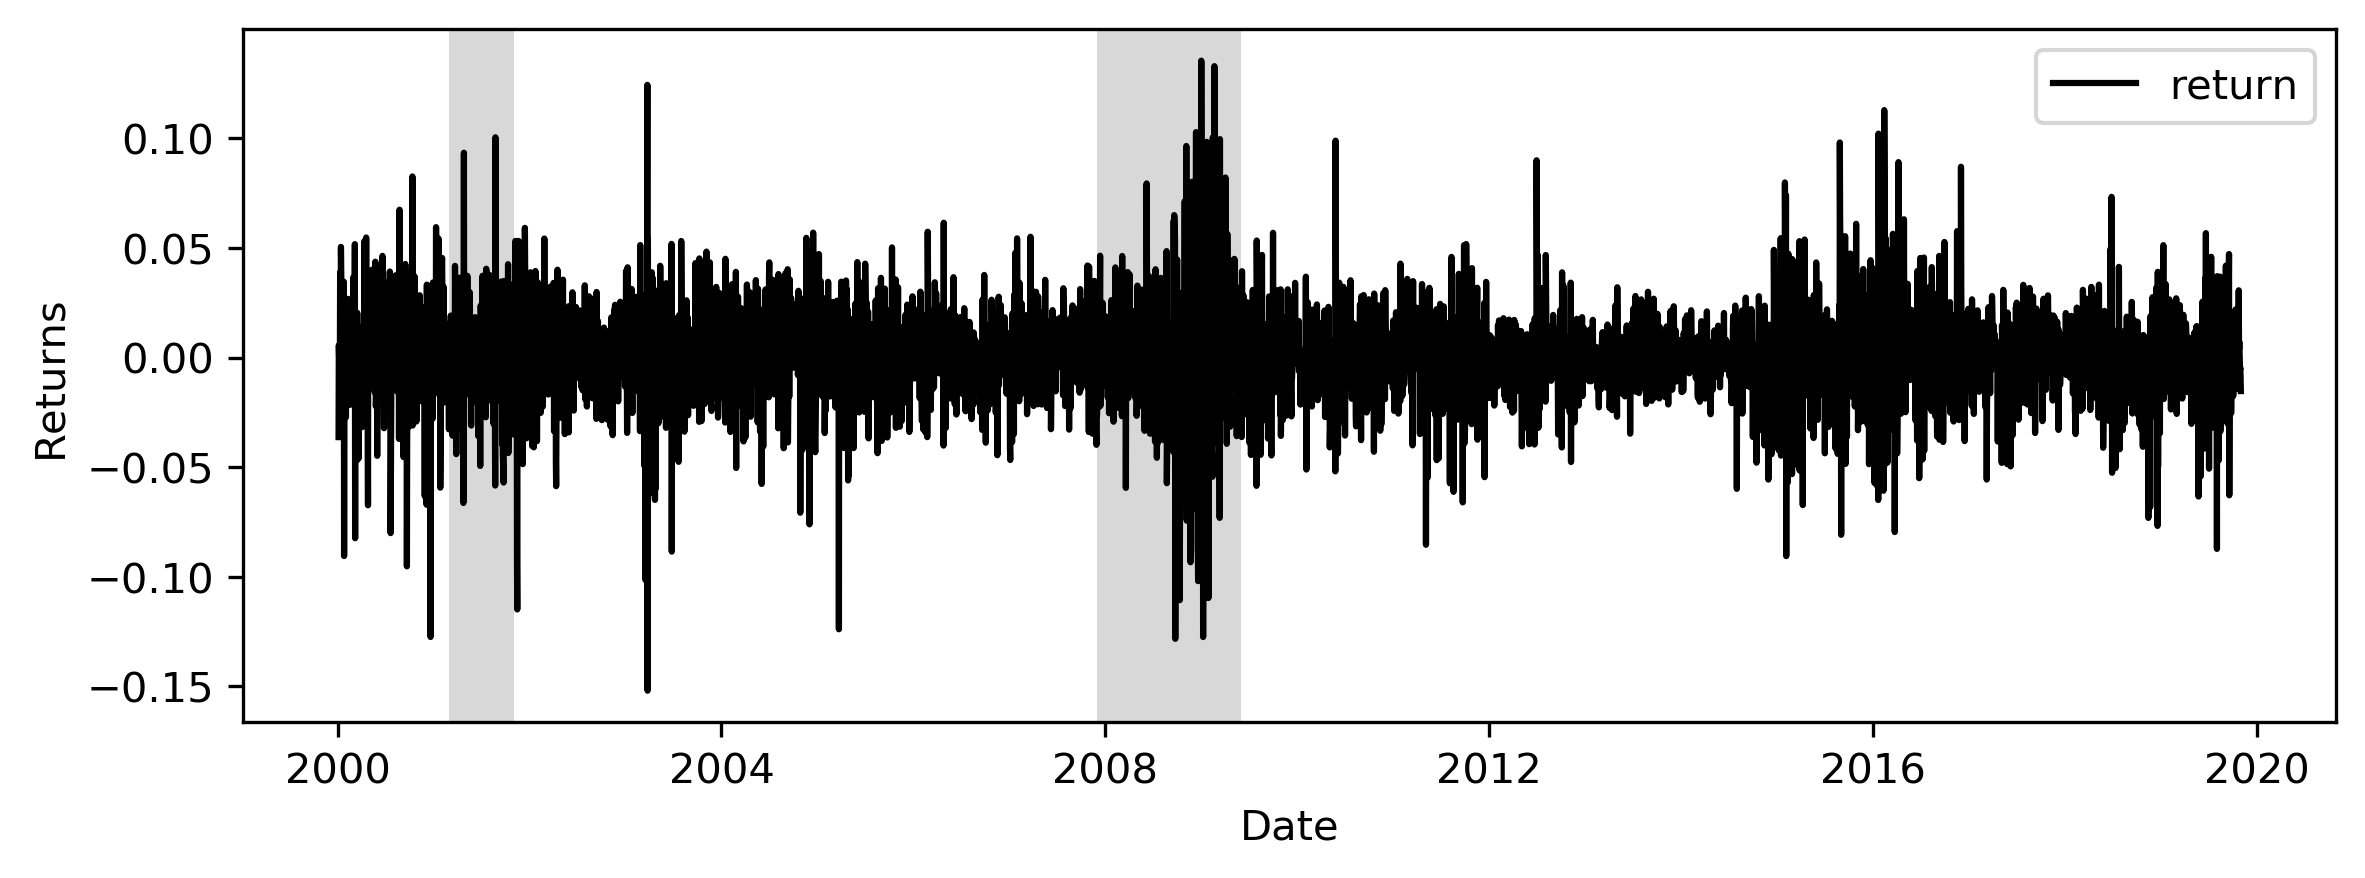
\includegraphics[width=\linewidth]{figures/wti_summary/returns.png}
	\end{figure}
	
	\par \textbf{The table of summary statistics below} suggests the mean return within each year are nearly zero. During periods of recessions, the average returns are below -2\%, the series becomes significantly more volatile as well. Given the high kurtosis between 2008 and 2009, one are more likely to encounter extreme returns, both positive and negative, during recession periods.
	\begin{table}[H]
		\small
		\centering
		\caption{Summary Statistics for Crude Oil Returns (Percentages)}
		\begin{tabular}{l|c c c c c c c c}
			\toprule
Year & Obs. & Mean & Median & Std. & Min & Max & $3^{rd}$ Moment & $4^{th}$ Moment \\
			\midrule
2000 & 249 & 0.03433 & 0.20148 & 2.61996 & -12.74152 & 8.26343 & -16.57663 & 304.18069 \\
2001 & 250 & -0.02409 & -0.04434 & 2.54058 & -11.48581 & 10.05107 & -1.05664 & 256.34141 \\
2002 & 250 & 0.15535 & 0.15221 & 1.70283 & -5.86460 & 5.43272 & -1.10096 & 30.47303 \\
2003 & 250 & 0.07861 & 0.13203 & 2.57315 & -15.19090 & 12.44253 & -15.23783 & 451.62566 \\
2004 & 249 & 0.08918 & 0.11605 & 2.08792 & -7.60501 & 5.70121 & -3.46945 & 76.28297 \\
2005 & 251 & 0.05257 & 0.11019 & 1.96717 & -12.39009 & 5.02715 & -7.95491 & 132.38058 \\
2006 & 249 & -0.00539 & 0.12995 & 1.58949 & -4.45214 & 6.15402 & 0.54160 & 25.74049 \\
2007 & 252 & 0.23400 & 0.09798 & 1.69800 & -4.66915 & 5.51381 & 0.67096 & 30.42035 \\
2008 & 253 & -0.29945 & -0.07920 & 3.34992 & -12.82672 & 13.54551 & -0.62036 & 705.61292 \\
2009 & 252 & 0.26537 & 0.19157 & 2.92040 & -12.74310 & 13.29544 & 7.30616 & 528.06699 \\
2010 & 252 & -0.02077 & 0.03198 & 1.74554 & -5.18874 & 9.89802 & 2.09087 & 63.31449 \\
2011 & 252 & 0.00583 & 0.10994 & 1.94170 & -8.53498 & 5.18170 & -5.06359 & 74.96618 \\
2012 & 252 & -0.04164 & 0.03600 & 1.51078 & -4.76060 & 9.00091 & 1.89035 & 44.44938 \\
2013 & 252 & 0.01455 & 0.04489 & 1.06690 & -3.46951 & 3.20999 & 0.06673 & 4.76023 \\
2014 & 252 & -0.16510 & -0.05343 & 1.36052 & -5.98638 & 4.91592 & -1.93871 & 21.11776 \\
2015 & 252 & -0.03610 & -0.25616 & 2.63361 & -9.05140 & 9.81397 & 4.40762 & 204.56338 \\
2016 & 252 & 0.20931 & 0.00000 & 2.79698 & -7.95603 & 11.28922 & 15.41866 & 313.23980 \\
2017 & 250 & 0.06564 & 0.17286 & 1.40987 & -5.56187 & 3.32016 & -2.44842 & 20.04256 \\
2018 & 249 & -0.10076 & 0.07393 & 1.81925 & -7.67683 & 7.33414 & -3.86867 & 69.95139 \\
2019 & 210 & 0.04359 & 0.10073 & 1.93931 & -8.72444 & 5.67862 & -4.83203 & 83.04972 \\
			\midrule
Total & 4978 & 0.02754 & 0.06307 & 2.15250 & -15.19090 & 13.54551 & -1.61083 & 174.47526 \\
			\bottomrule
		\end{tabular}
	\end{table}

	\begin{figure}[H]
		\small
		\centering
		\caption{ACF and PACF for Crude Oil Returns}
		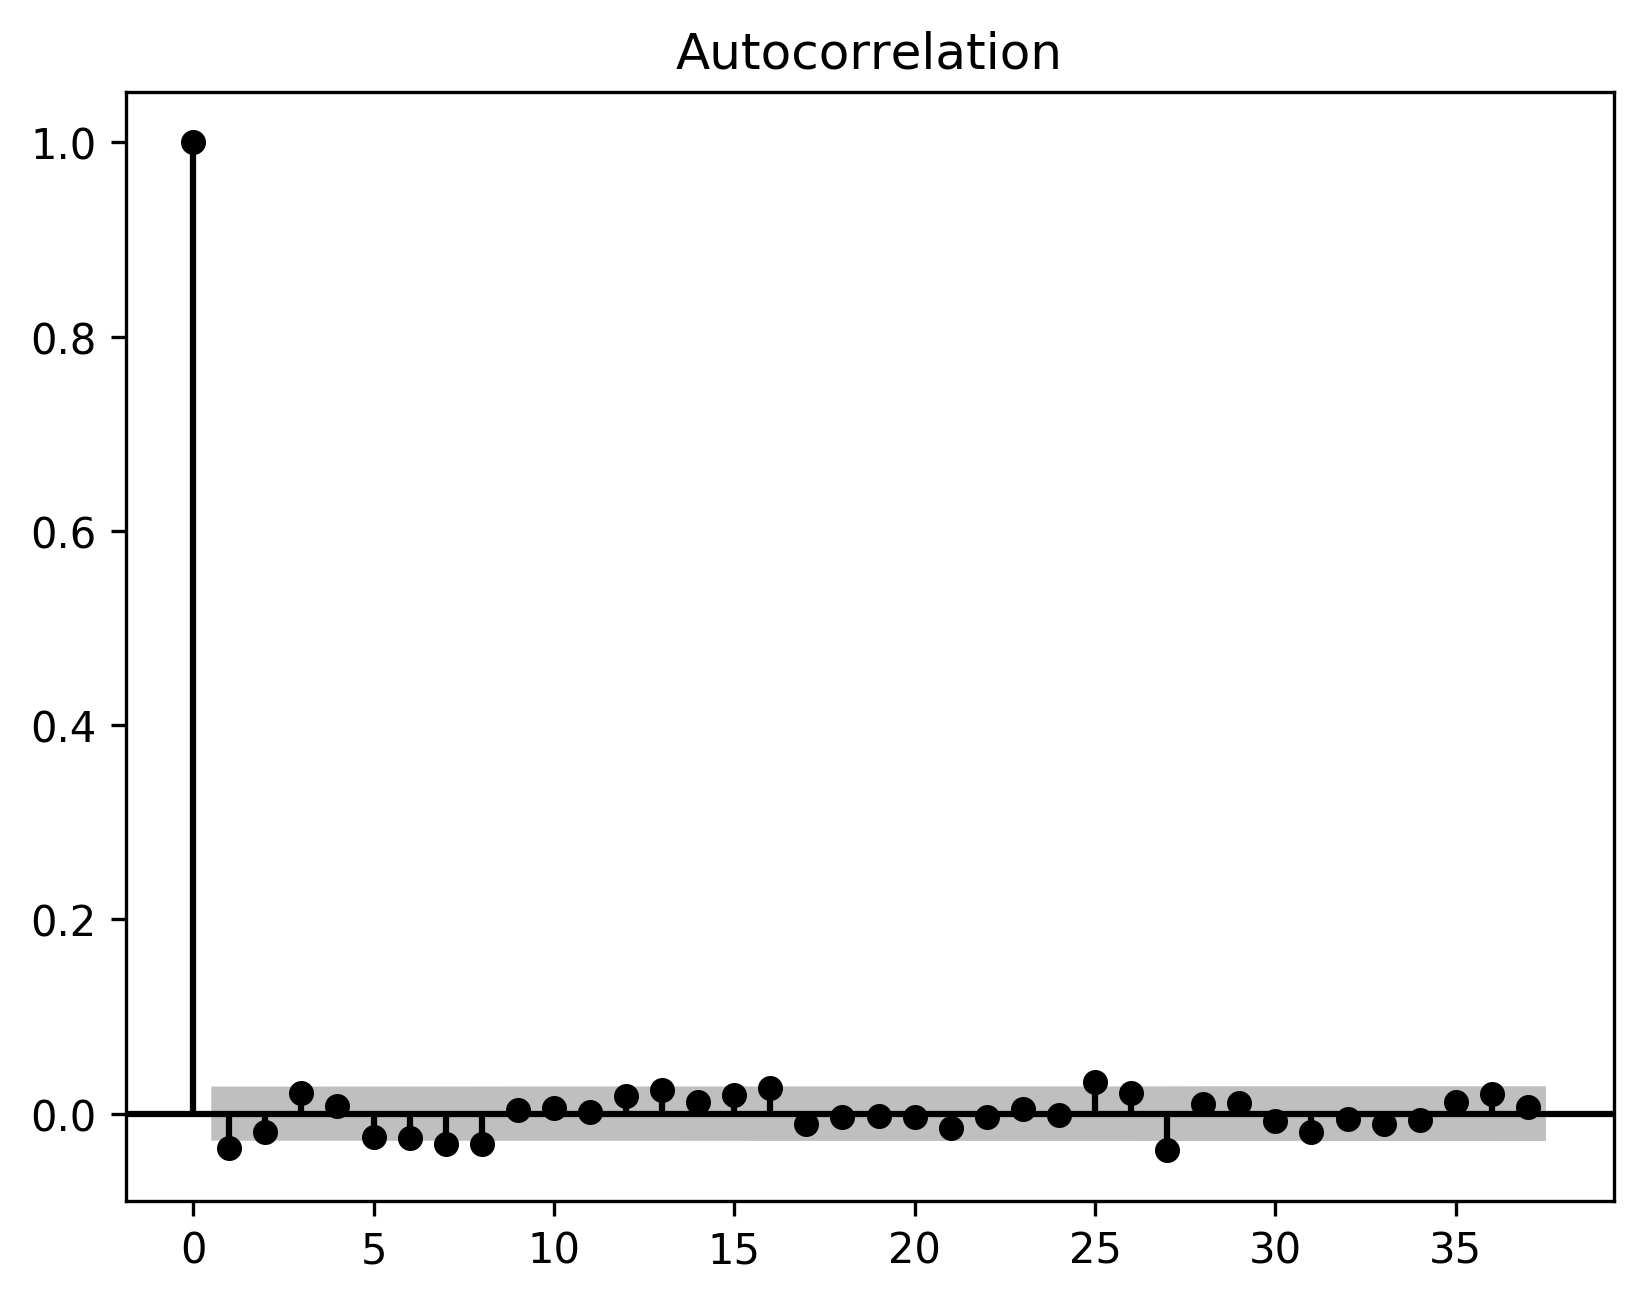
\includegraphics[width=0.45\linewidth]{figures/wti_summary/returns_acf.png}
		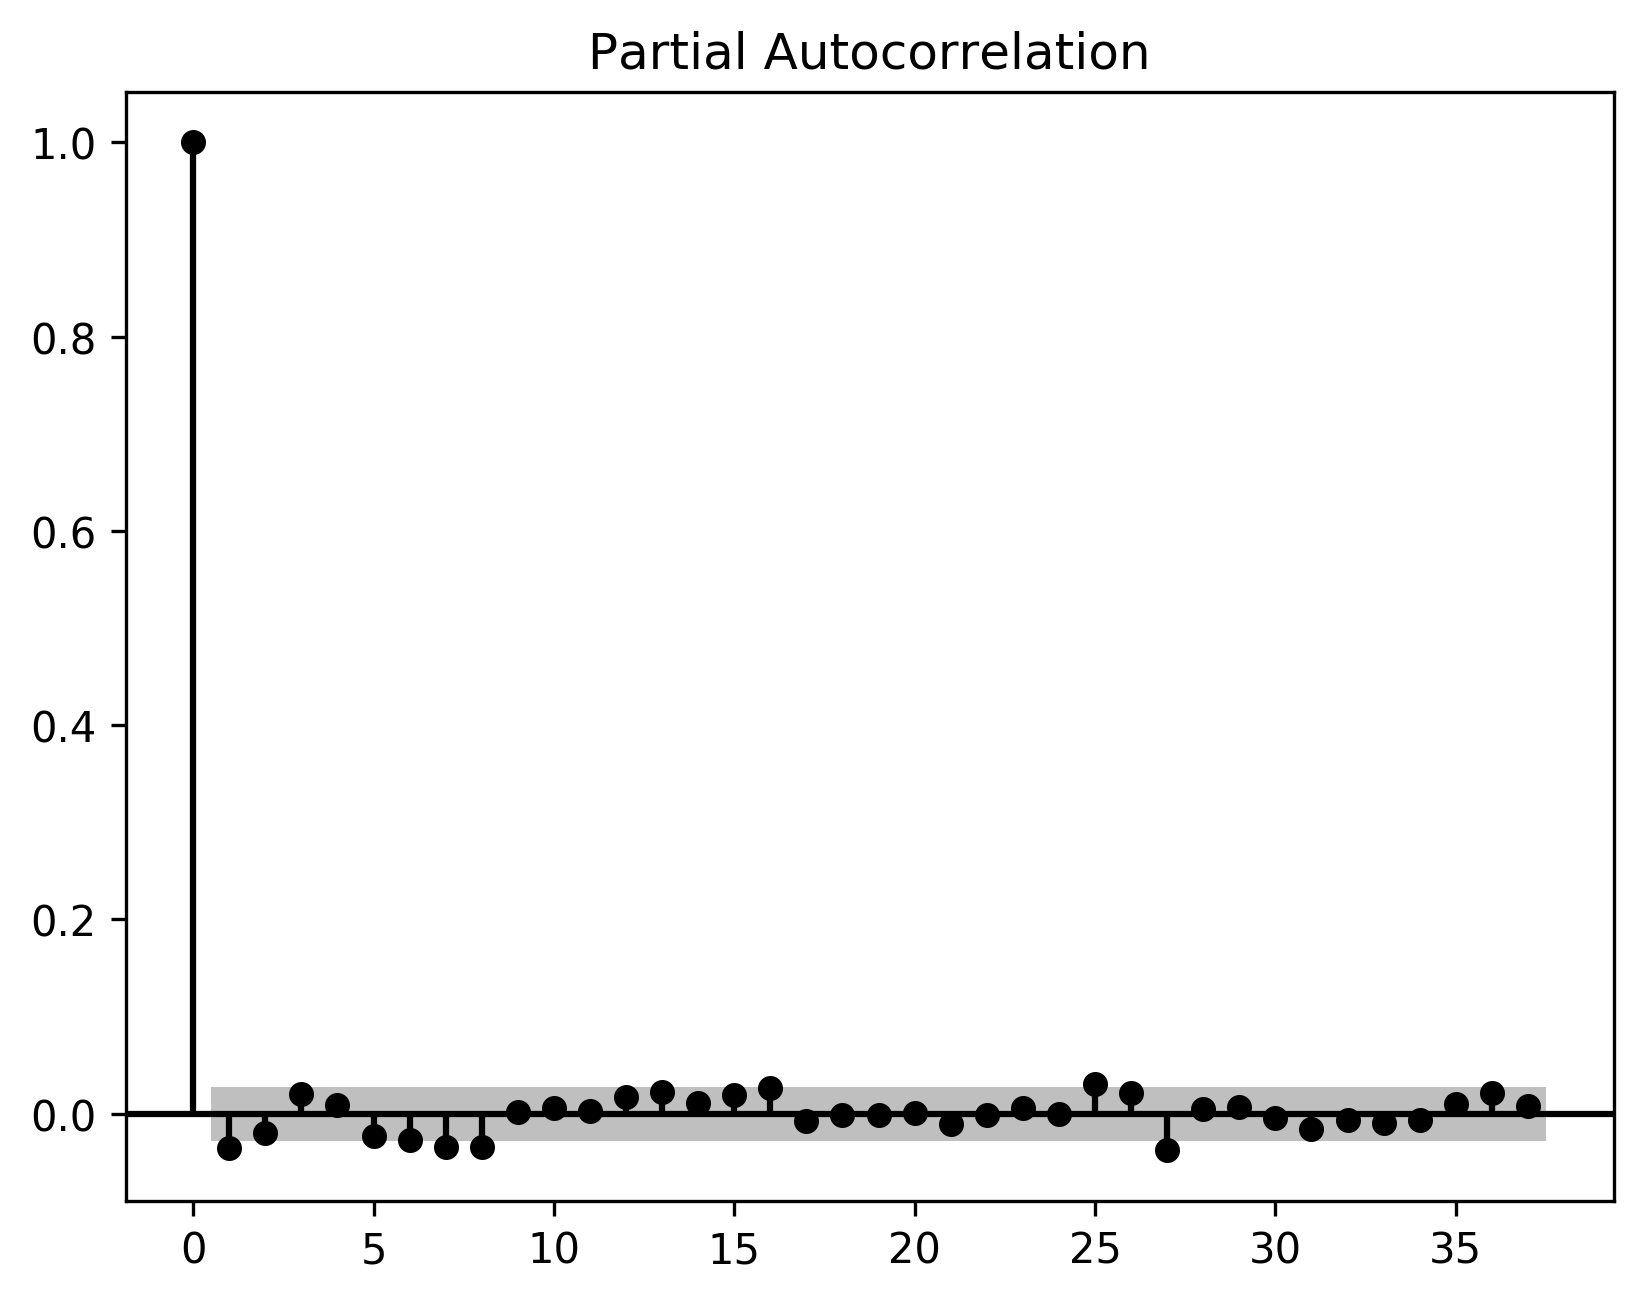
\includegraphics[width=0.45\linewidth]{figures/wti_summary/returns_pacf.png}
	\end{figure}
	
	\par For both autocorrelation function (ACF) and partial autocorrelation function (PACF), only a few lags are statistically significant, which suggests the impotency  of linear models on this problem.
	\todo{Stopped here}
	\begin{figure}[H]
		\centering
		\small
		\caption{Distribution of Crude Oil Returns}
		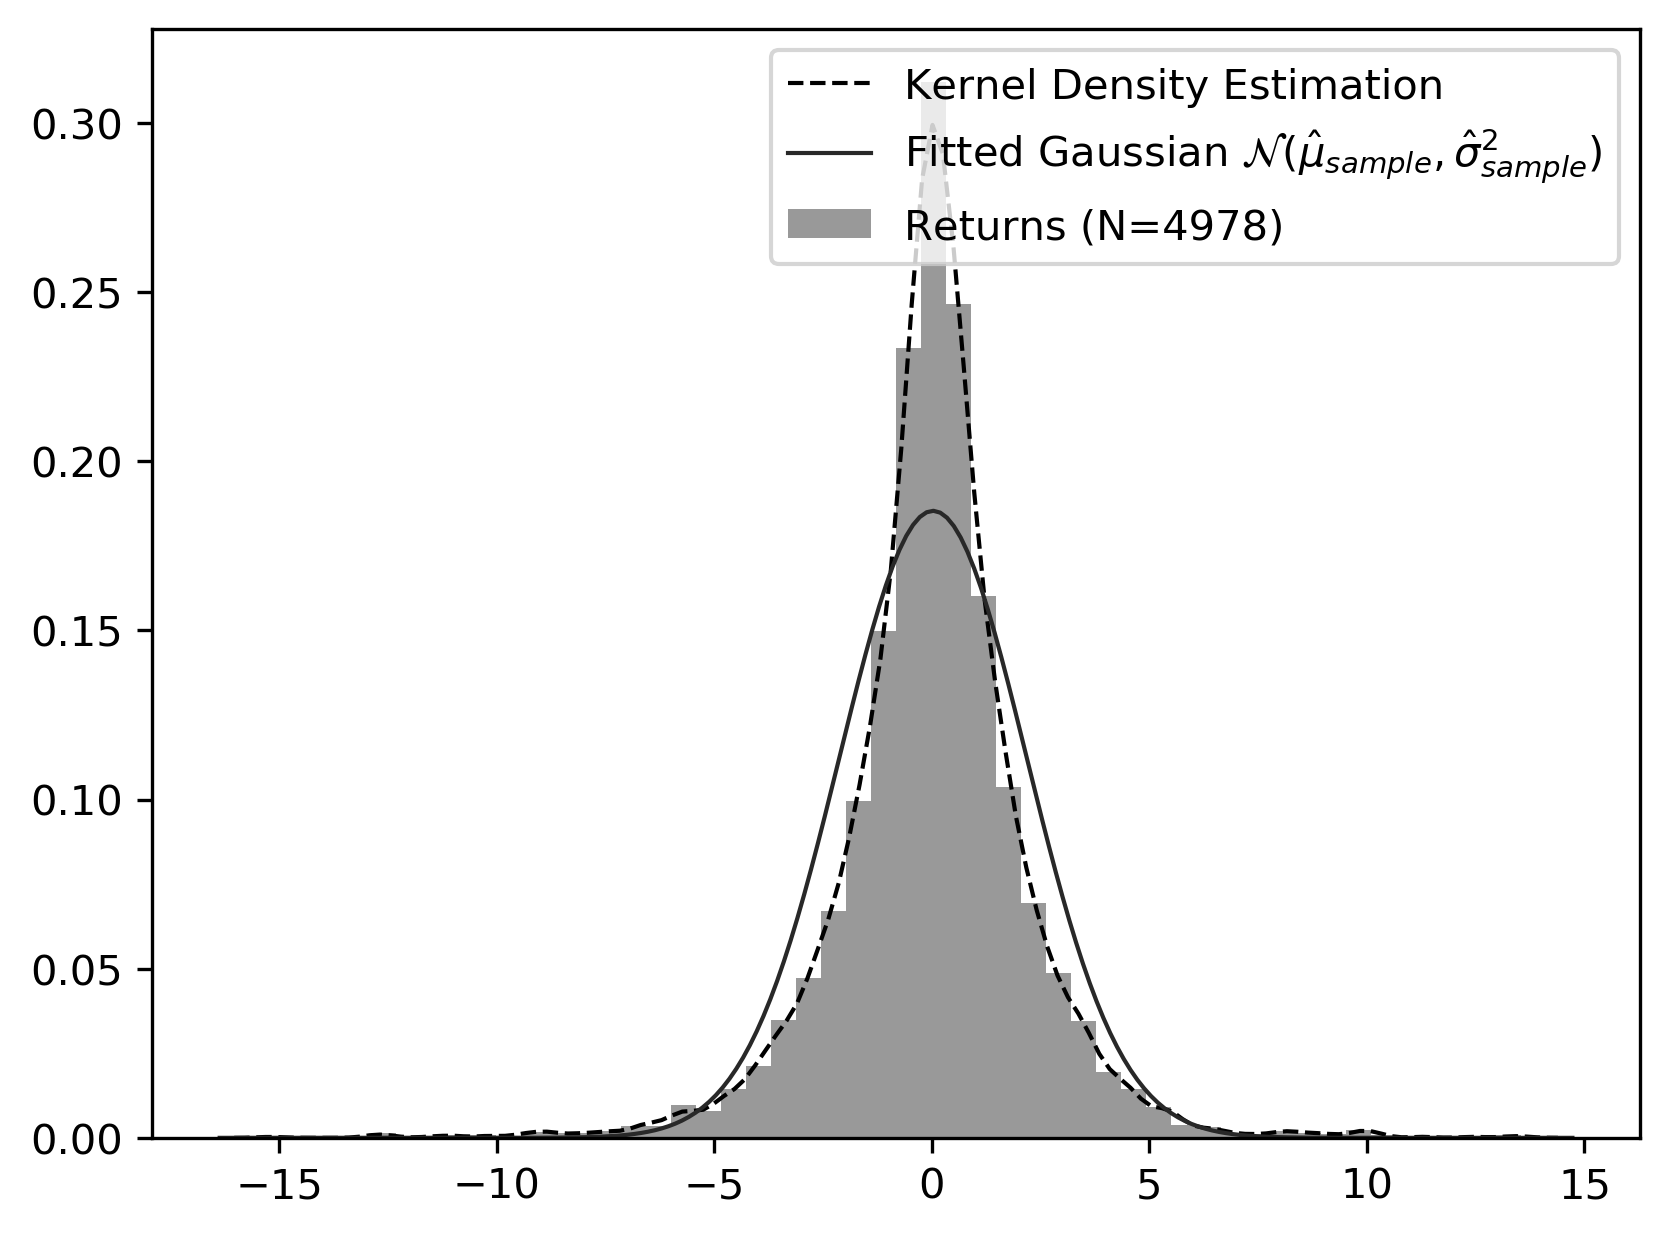
\includegraphics{figures/wti_summary/return_hist.png}
	\end{figure}
 
	\subsection{Day of the Week Effect in Crude Oil Dataset}
	\subsubsection{Difference in Returns across the Week}
	\paragraph{} Gibbons and Hess' work examined returns on stocks from S\&P 500, Dow Jones 30, and Treasury Bills. They found strong negative mean returns on Monday compared with other weekdays.
	The seasonality persisted even after taking market adjustment measures, such as using mean-adjusted returns instead \cite{Hess1981}. 
	Analysis in my paper unveils a similar daily seasonality presents in crude oil returns as well.
	\textbf{Panels in the figure below} demonstrate the empirical distributions of returns on each day of the week. We can see that Mondays and Wednesdays have relatively larger variances, which again matches Gibbons and Hess' observations.
	\begin{figure}[H]
		\centering
		\small
		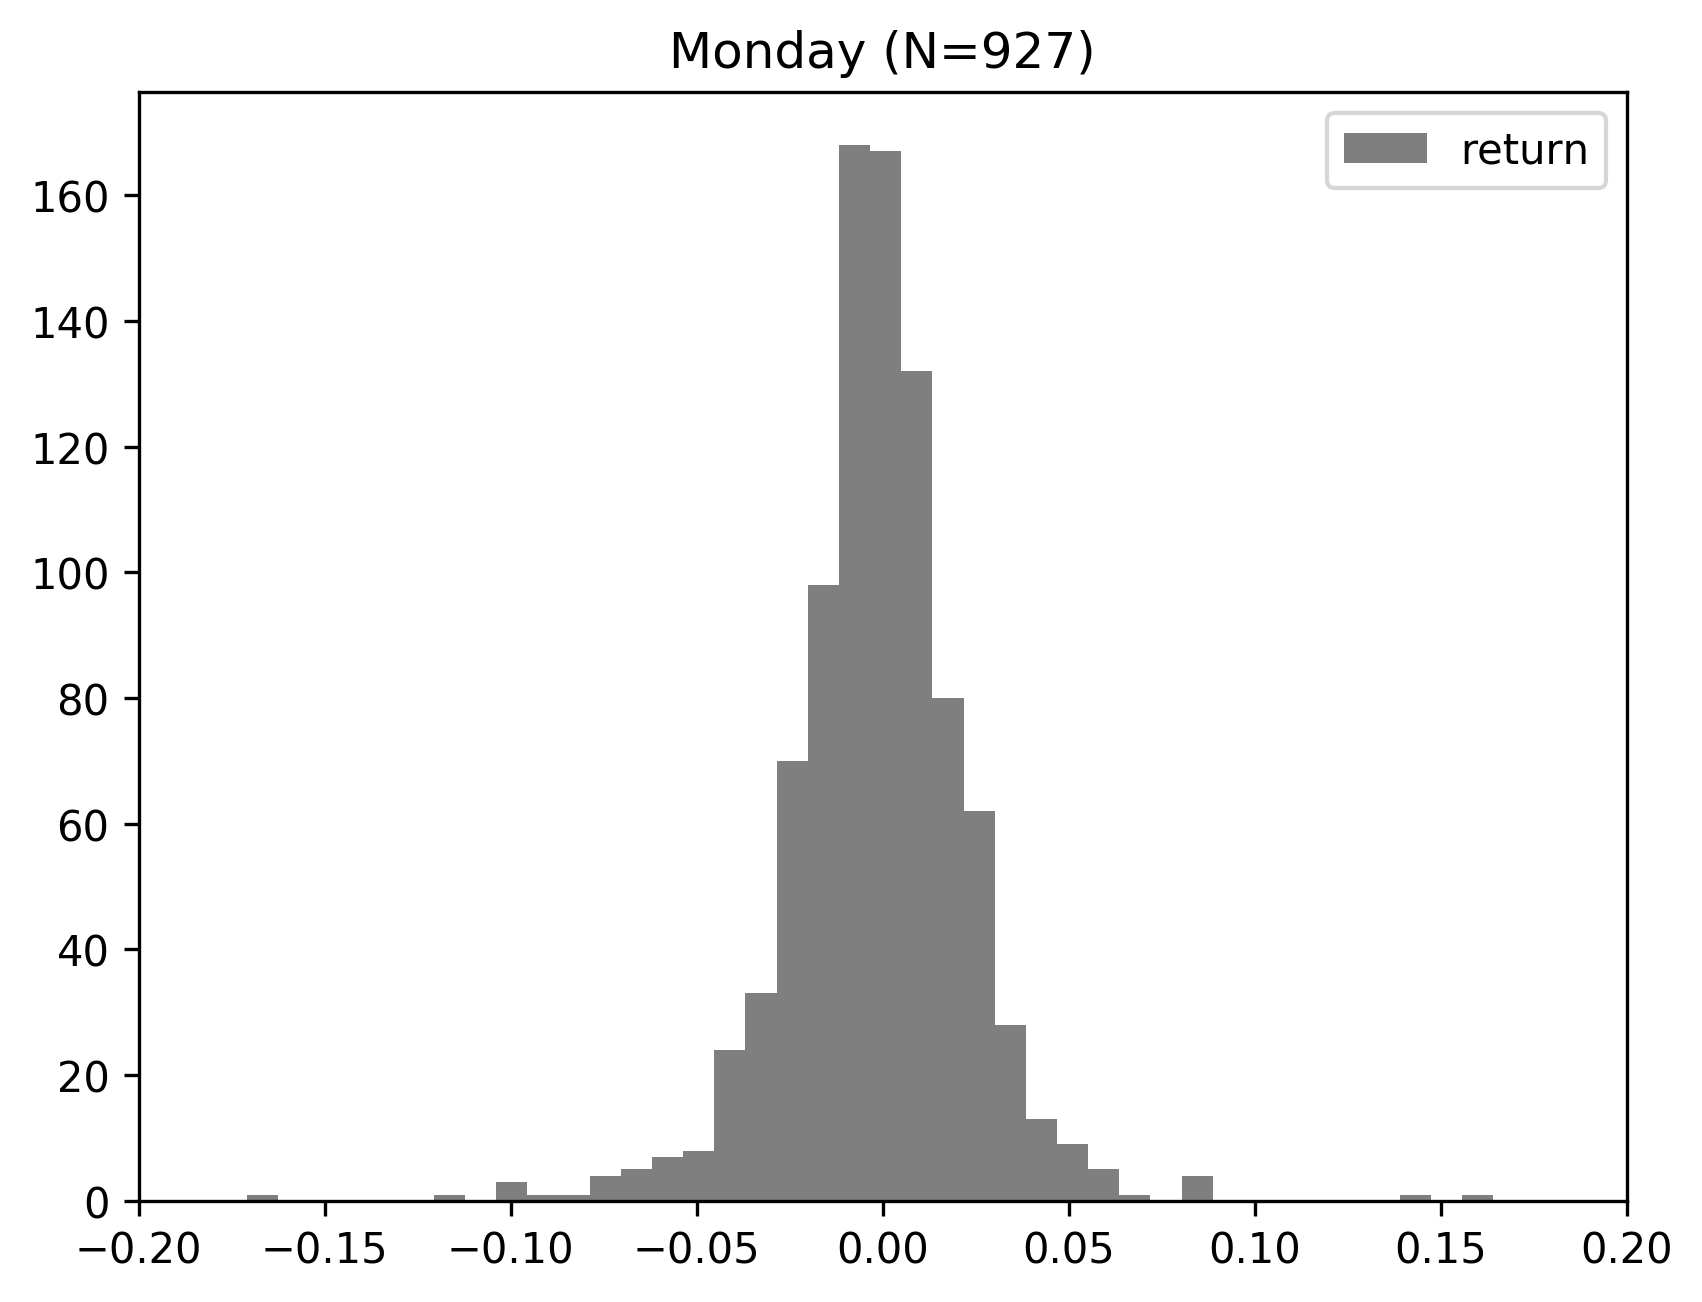
\includegraphics[width=0.45\linewidth]{figures/day_of_week_effect/dist_returns_Monday.png}
		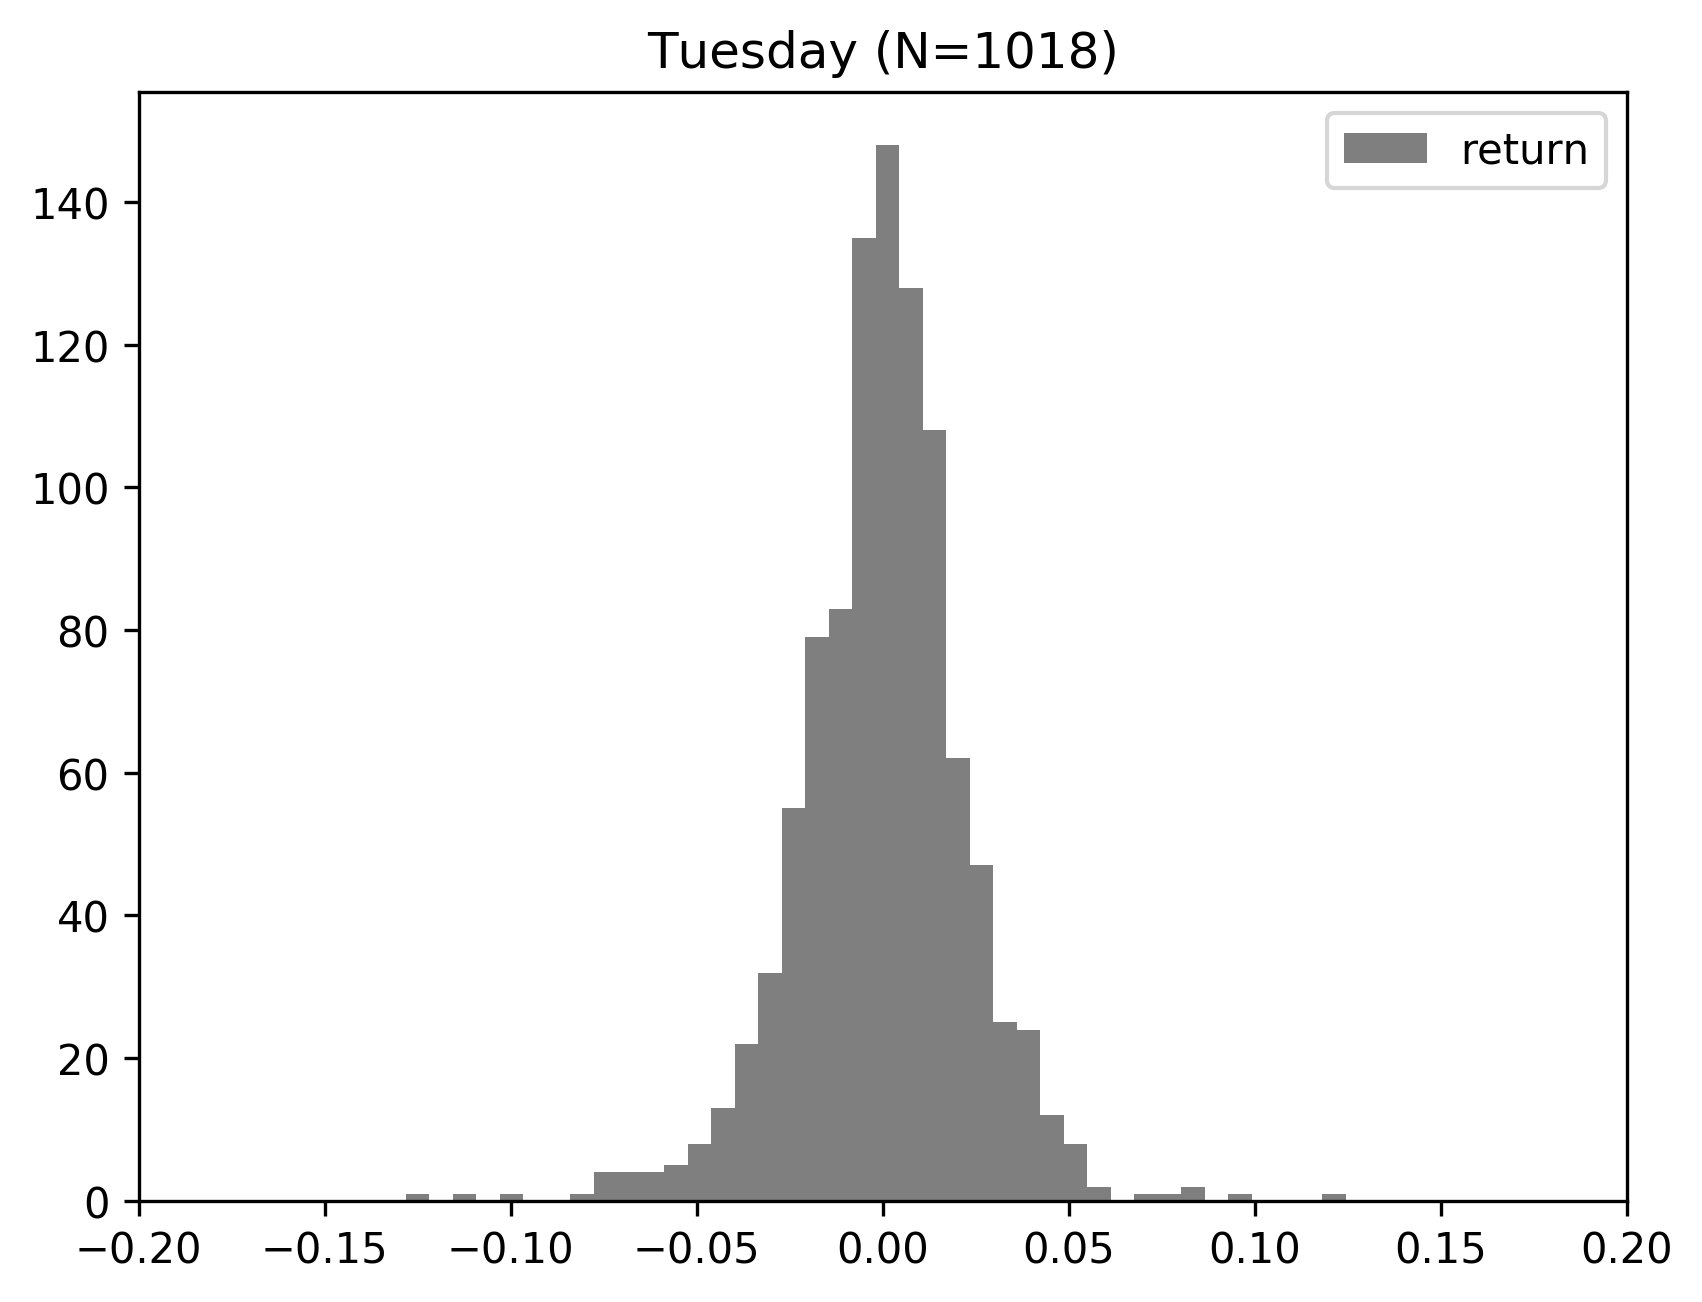
\includegraphics[width=0.45\linewidth]{figures/day_of_week_effect/dist_returns_Tuesday.png}
		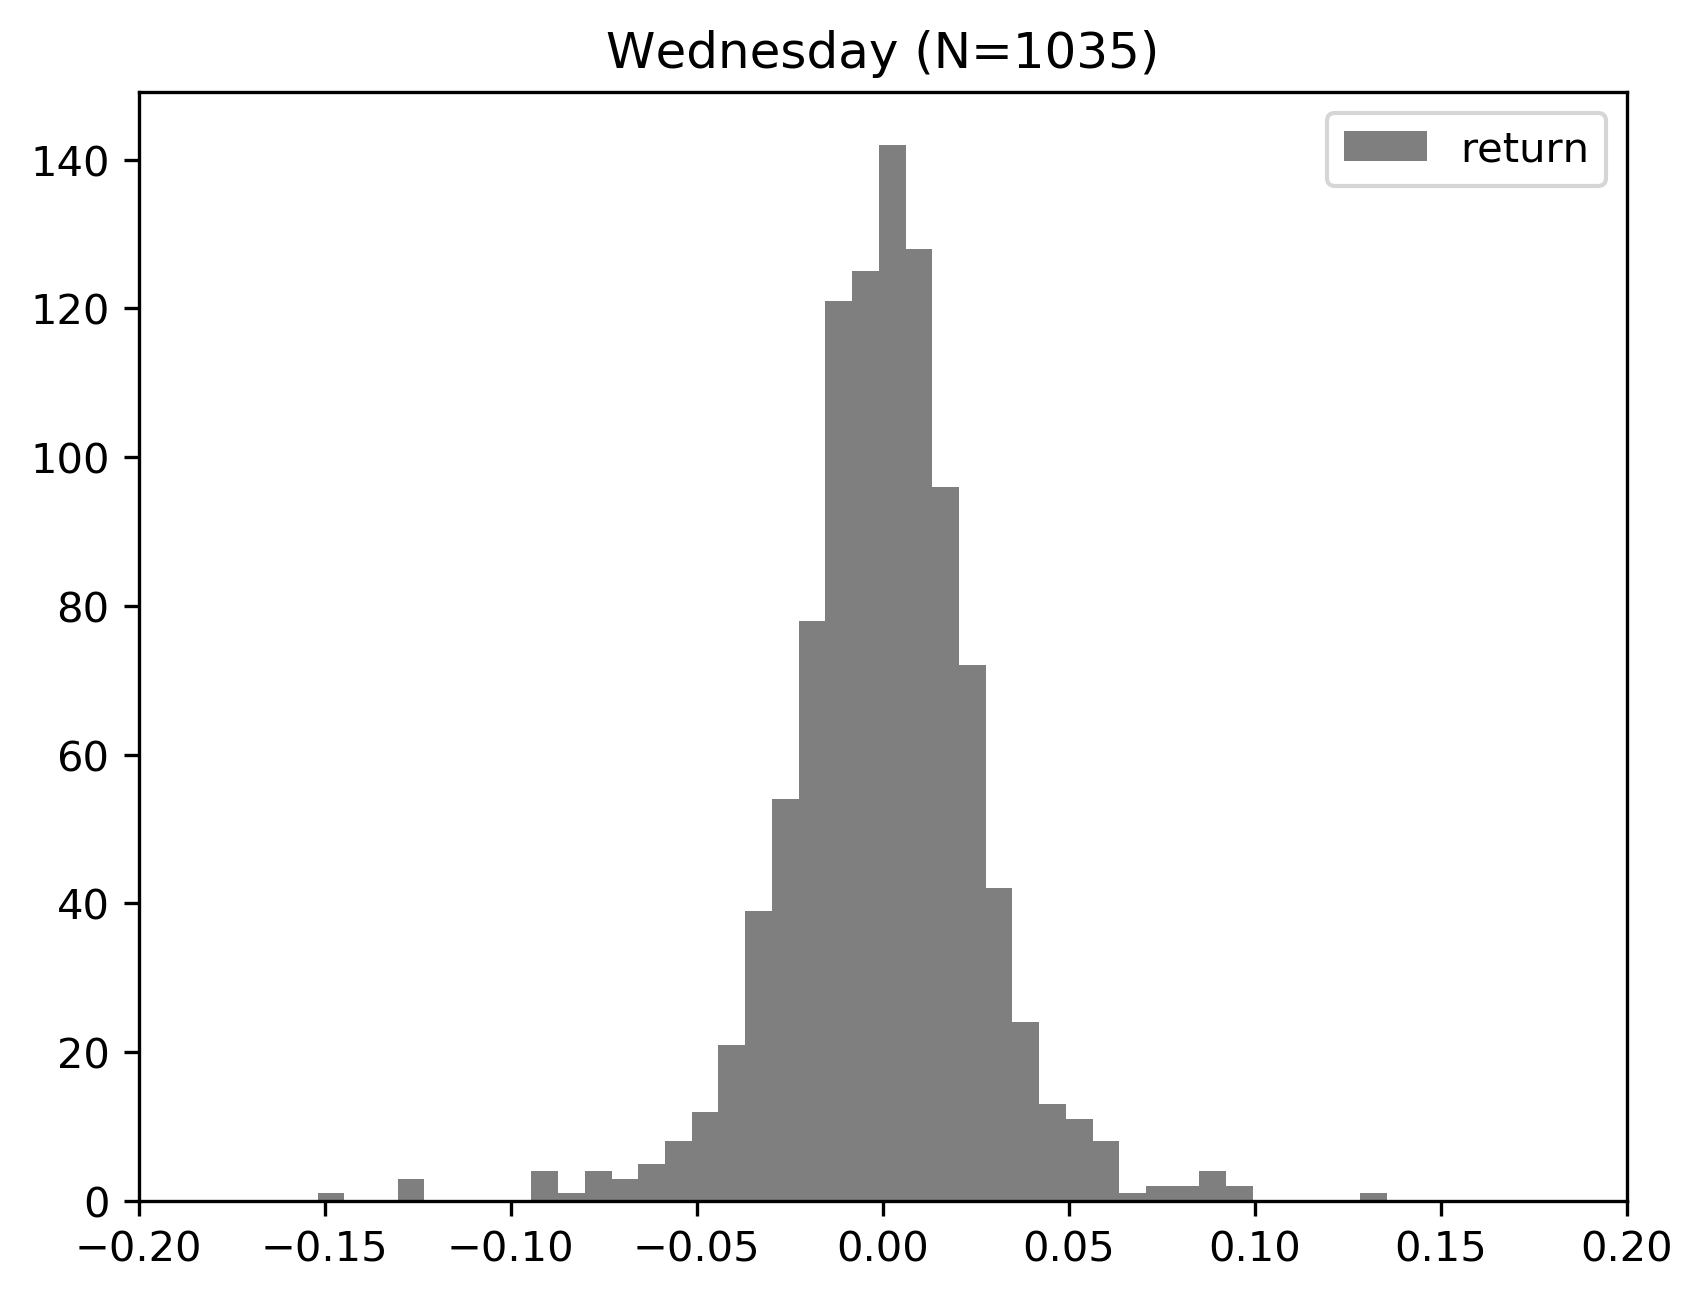
\includegraphics[width=0.45\linewidth]{figures/day_of_week_effect/dist_returns_Wednesday.png}
		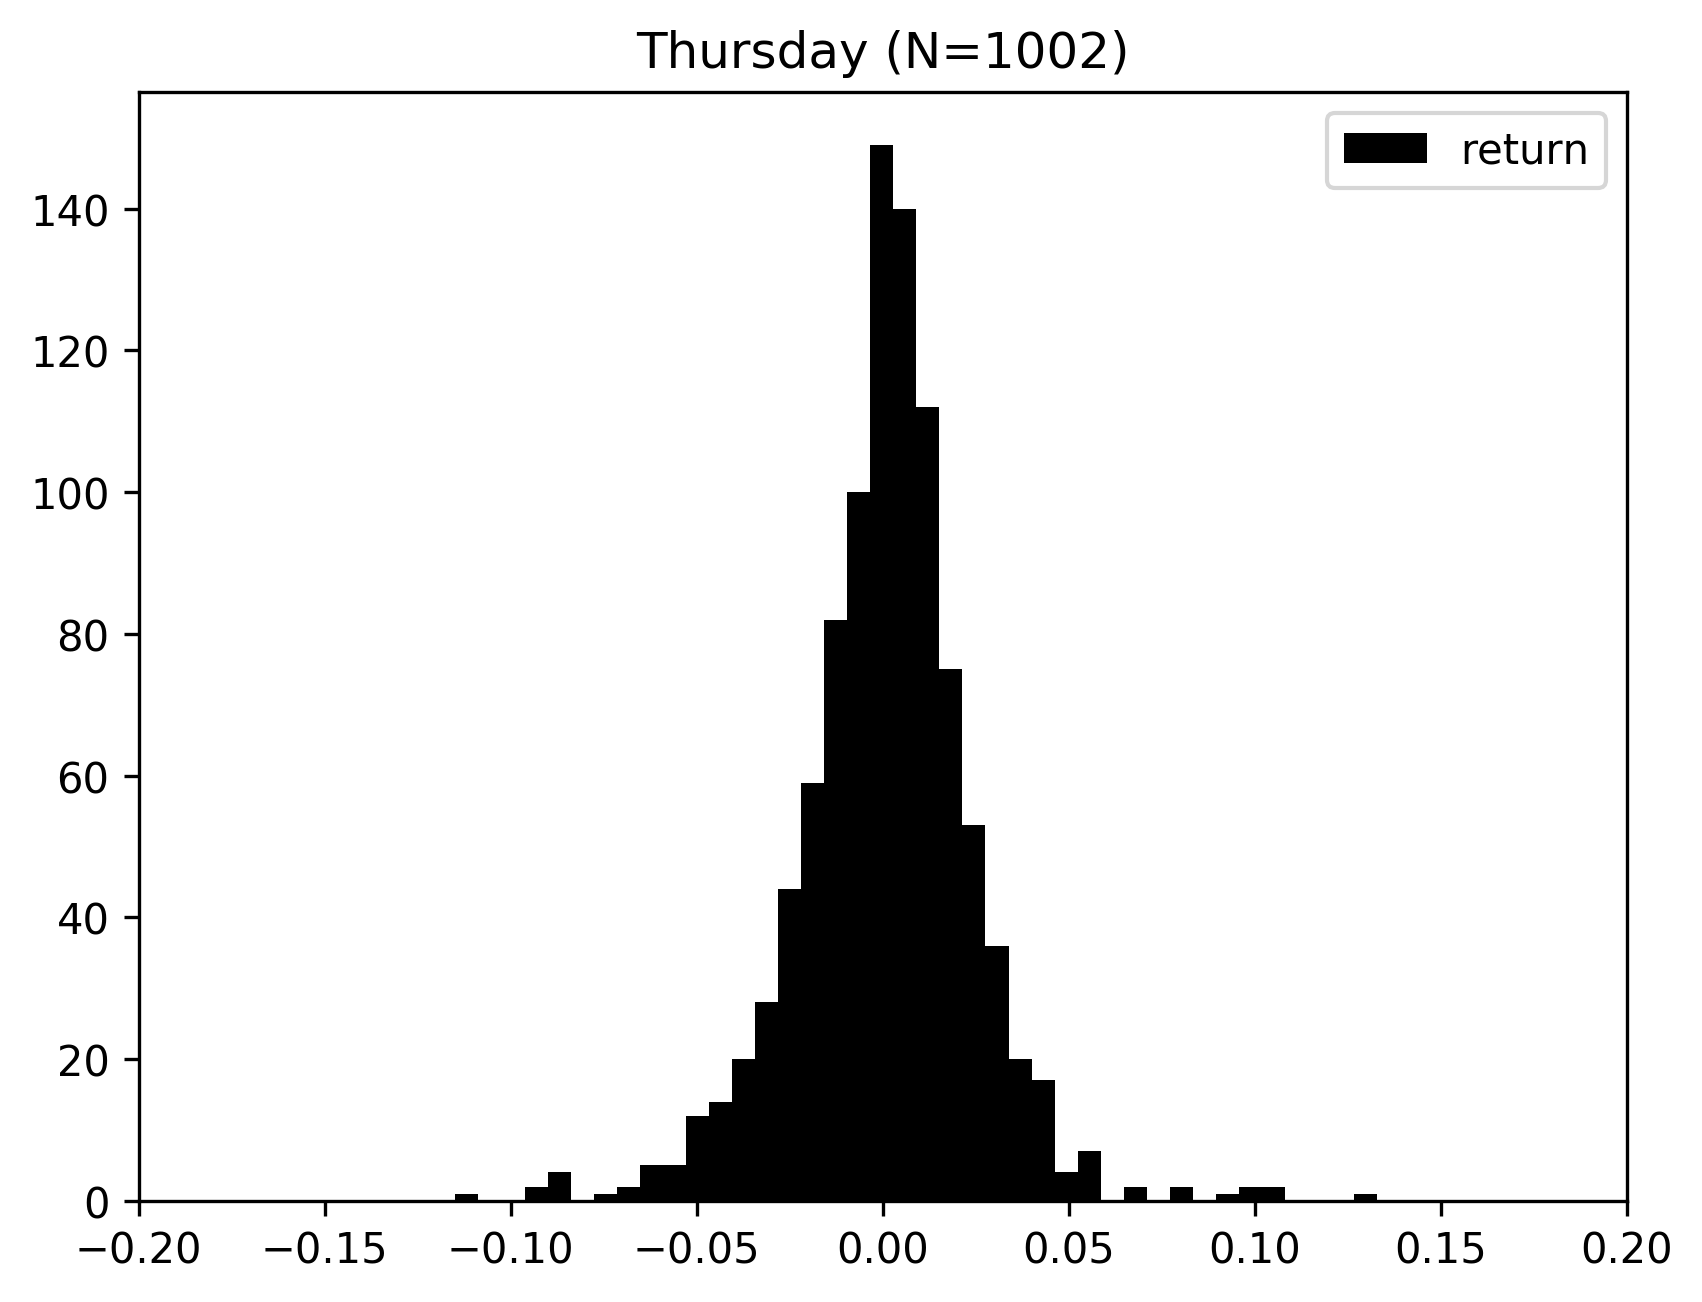
\includegraphics[width=0.45\linewidth]{figures/day_of_week_effect/dist_returns_Thursday.png}
		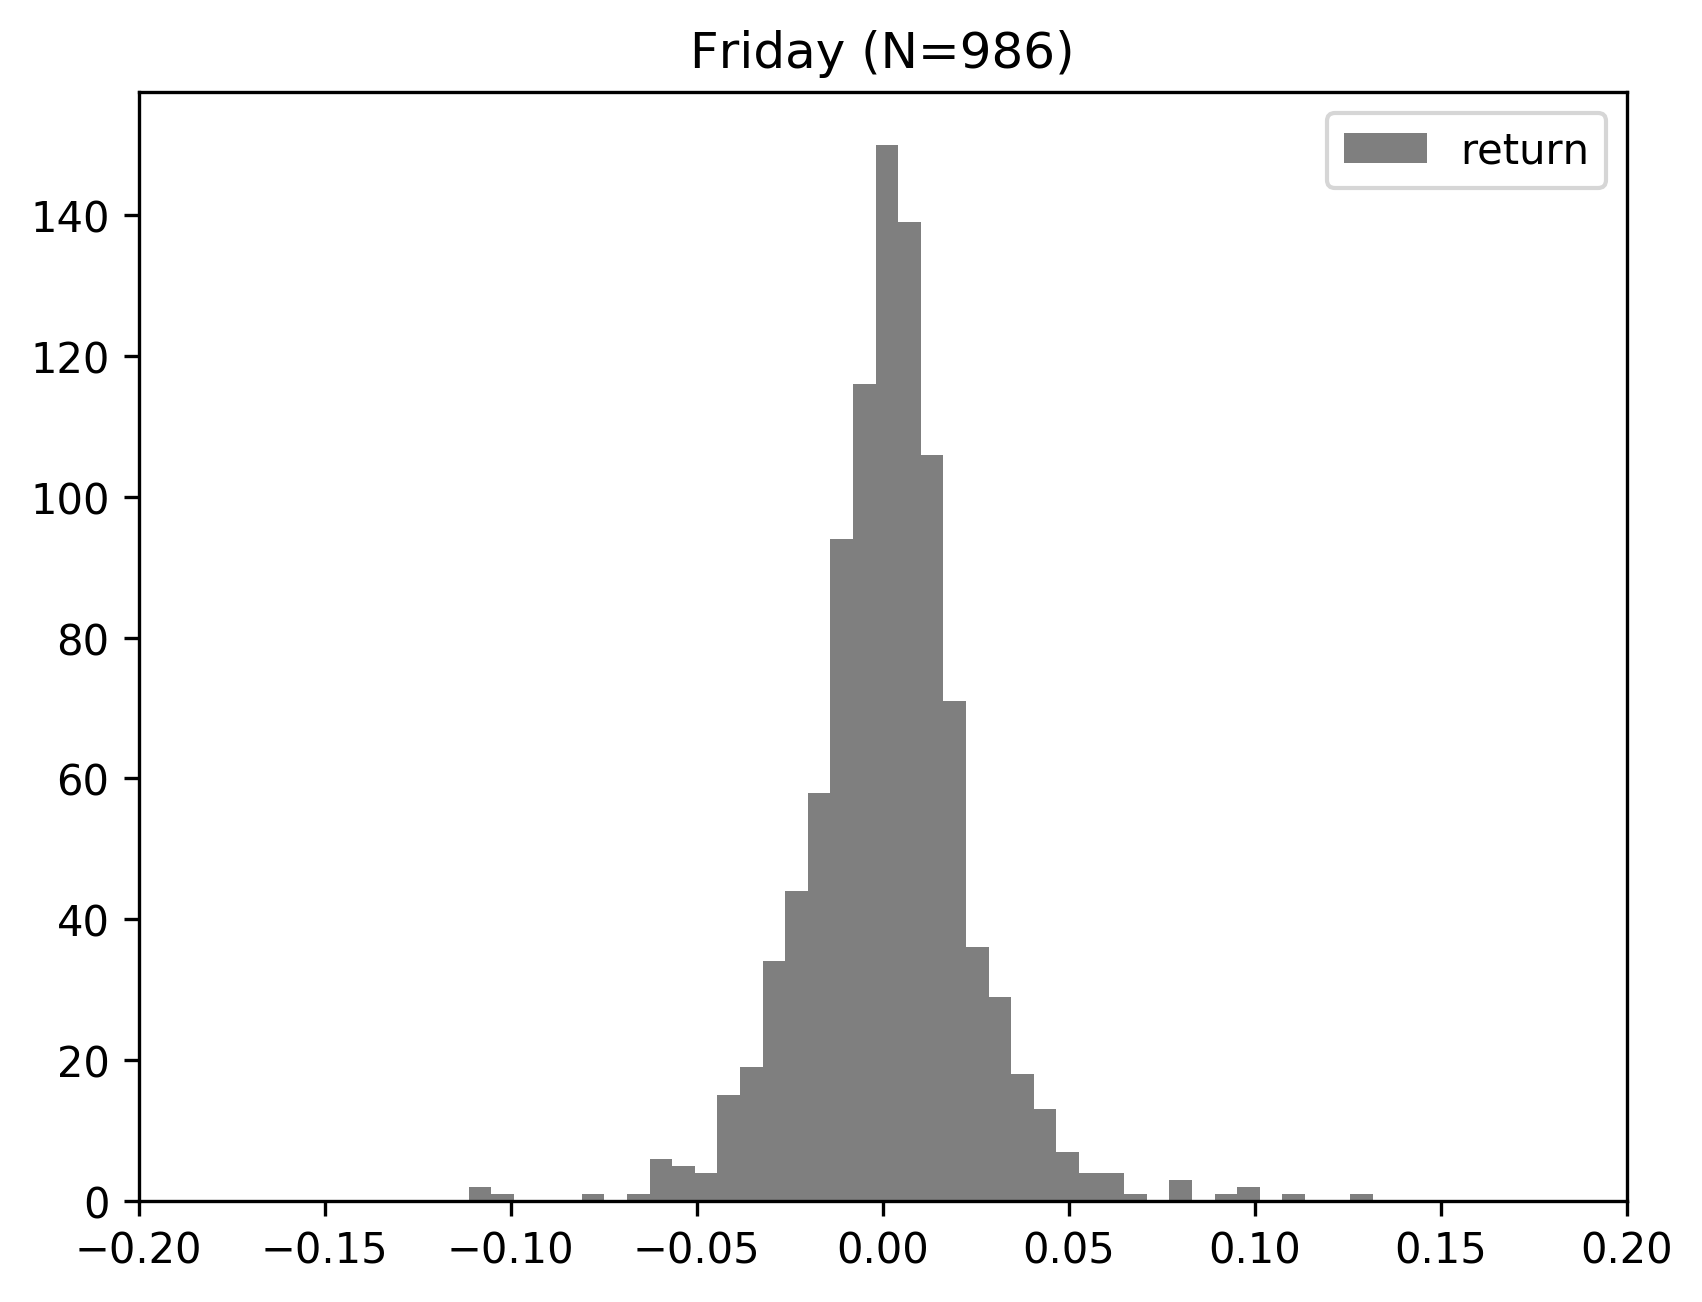
\includegraphics[width=0.45\linewidth]{figures/day_of_week_effect/dist_returns_Friday.png}
		\caption{Crude oil returns on each weekday. Weekend data are not available in the daily dataset provided by U.S. Energy Information Administration (EIA). $N$s within parentheses in figure titles denote the number of observations. See appendix for distributions of crude oil prices.}
	\end{figure}

	\par The \textbf{two tables} below provide summary statistics for prices and returns on each day. It turns out that Monday is the only weekday with a mean return significantly less than zero.
%	\begin{table}[H]
%		\small
%		\centering
%		\begin{tabular}{l|c c c c}
%			\toprule
%			Day of the week & Num. Obs. & Mean & Std. & $3^{rd}$ Moment \\
%			\midrule
%Monday & 931 & -0.001 & 0.008 & -0.0000001 \\
%Tuesday & 1,023 & -0.000 & 0.021 & -0.0000033 \\
%Wednesday & 1,027 & -0.000 & 0.027 & -0.0000061 \\
%Thursday & 1,007 & 0.001 & 0.024 & -0.0000005 \\
%Friday & 990 & 0.002 & 0.022 & 0.0000013 \\
%			\midrule
%			Total & 4,978 & & & \\
%			\bottomrule
%		\end{tabular}
%		\caption{Summary statistics of crude oil prices on each day of week}
%	\end{table}

	\begin{table}[H]
		\small
		\centering
		\begin{tabular}{l|c c c c}
			\toprule
			Day of the week & Num. Obs. & Mean ($P$-Value) & Std. & $3^{rd}$ Moment \\
			\midrule
			Monday & 927 & \textbf{-0.002 (0.049)} & 0.025 & -0.0000019 \\
			Tuesday & 1018 & -0.000 (0.900) & 0.023 & -0.0000031 \\
			Wednesday & 1022 & 0.000 (0.884) & 0.027 & -0.0000054 \\
			Thursday & 1002 & 0.001 (0.361) & 0.024 & -0.0000006 \\
			Friday & 986 & \textbf{0.002 (0.0311)} & 0.023 & 0.0000021 \\
			\midrule
			Total & 4955 & & & \\
			\bottomrule
		\end{tabular}
		\caption{Summary statistics of crude oil returns on each day of week. The first day (January 1, 2000) of the oil price dataset was Saturday, and the observation on the following Monday (January 3) was missing. Hence, the return on Tuesday (January 4) could not be computed because it was the first trading day in this dataset, and there are only 1018 Tuesdays in the dataset of returns. A value of $-0.000$ indicates a negative value with magnitude less than $0.0005$. $P$-values are calculated in a two-tailed $t$-test with $\mu_0 = 0$. Bold fonts indicate statistically significance at level $\alpha=0.05$.}
	\end{table}
	
	\subsubsection{Kolmogorov-Smirnov test for Distributional Similarities}
	\par Smirnov developed a non-parametric method of testing the equality between two continuous distributions, with CDFs $F(x)$ and $G(x)$ respectively, \cite{Smirnov1939}. Refer to Hodges' work for a detailed review on the Kolmogorov-Smirnov test \cite{Hodges1957}. I am using the two-tailed version of Kolmogorov-Smirnov test to check whether distributions of two different days are similar.
	Given two datasets, take returns on Mondays and Tuesdays for example, the null hypothesis says those two datasets are drawn from the same distribution, and the alternative says they are from different distributions \footnote{Different alternative hypotheses can be used in Kolmogorov–Smirnov test: i) $H_1: F(x) \geq G(x)$, ii) $H_1: F(x) \leq G(x)$, and iii) $H_1: F(x) \neq G(x)$. This paper is using the third (two-tailed) alternative hypothesis.}.
	Firstly, the Kolmogorov–Smirnov test constructs the empirical CDFs $F_{Mon, 927}(x)$ and $F_{Tue, 1018}(x)$ from the dataset. Then, the Kolmogorov–Smirnov statistic measures the maximum discrepancy between two distribution functions, which is
	\begin{align}
		D := \sup_x \abs{F_{Mon, 927}(x) - F_{Tue, 1018}(x)} \in [0, 1]
	\end{align}
	A smaller $D$-statistic implies stronger distributional similarity between two distributions. For instance, when $F_{Mon, 927}(x)$ and $F_{Tue, 1018}(x)$ are exactly the same, the $D$-statistic is zero. In contrast, let $X=0$ and $Y=1$ be two deterministic random variables, in this case, $D_{X, Y} = 1$.\\
	The test rejects $H_0$ at a significance level of $\alpha$ if 
	\begin{align}
		D > \sqrt{-\frac{1}{2} \ln \frac{\alpha}{2}} \sqrt{\frac{n+m}{nm}}
	\end{align}
	where $m$ and $n$ denote sizes of two datasets.
	\begin{table}[H]
		\small
		\centering
		\begin{tabular}{l|c|c|c|c|c}
			\toprule
			$D$-Statistic ($P$-Value) & Monday & Tuesday & Wednesday & Thursday & Friday \\
			\midrule
Monday & 0.000(1.000) & \textbf{0.193(0.000)} &  \textbf{0.243(0.000)} &  \textbf{0.189(0.000)} &  \textbf{0.180(0.000)} \\
Tuesday & &  0.000(1.000) &  0.064(0.030) &  0.064(0.030) &  0.071(0.010) \\
Wednesday & & &  0.000(1.000) &  0.058(0.062) &  0.084(0.001) \\
Thursday & & & &  0.000(1.000) &  0.030(0.729) \\
Friday & & & & &  0.000(1.000) \\
			\bottomrule
		\end{tabular}
		\caption{The Kolmogorov-Smirnov $D$-Statistic for all pairs of distributions. Bold font indicates the null hypothesis is rejected at a significance level of 0.01, which implies discrepancy in distributions.}
	\end{table}
	\textbf{The table above} presents the Kolmogorov-Smirnov $D$-Statistic for distributions of every pairs of days. At a significance level of 0.05, we can see that Mondays follow a distribution significantly different from distributions of other weekdays follow. Because the dataset does not contain weekend data, returns on Mondays is always computed using the difference between log prices on Monday and the previous Friday (Thursday if Friday is not a trading day and so on). Therefore, returns associated with Mondays pick the weekend effect. In fact, the distribution of returns on Mondays (over weekends) is the only one with negative mean among distributions of all five days.

	\subsection{News and Sentiment Datasets}
	\paragraph{} The event sentiment dataset from RavenPack News Analytics (RPNA) tracks and analyzes all information of companies, organizations, countries, commodities, and currencies from four major sources: Dow Jones Newswires, Wall Street Journal, Barron’s and MarketWatch.
	\par The dataset covers events from January 1, 2000, to September 30, 2019. RavenPack records the exact date and coordinated universal time (UTC) when each news is published.s
	\par For each piece of news, the dataset links it to a unique entity name attribute. To filter out noise data less relevant to crude oil returns, this paper selects the subset of news with crude oil topic. There are 106, 960 entries from the original dataset left, lead to 15 events per day on average. In the figure below, panel A presents a distribution of ESS for all news related to crude oil in the time span of 20 years and panel B shows all distributions of events within each year.

	\par Moreover, the dataset categorizes each event following the RavenPack taxonomy.
	\begin{figure}[H]
		\centering
		\small
		\begin{enumerate}[(i)]
			\item topic;
			\item group;
			\item type;
			\item sub-type;
			\item property;
			\item category: fine details.
		\end{enumerate}
		\caption{Ravenpack taxonomy}
	\end{figure}
	\todo{Add examples of each level.} \todo{Add definitions of each level.}
	\par To proxy the potential economic impact upon news arrival and afterwards, Ravenpack assigns each piece of news an Event Sentiment Score (ESS) between 0 and 100 using an algorithm combines results from surveying financial experts and pattern matching. An ESS of 100 indicates extreme positive short-term positive financial or economic impact. In contrast, a 0 ESS score indicates extreme negative impact. And a ESS of 50 indicates exact neutral news. From this point, scores are normalized by subtracting 50, so that the sign of normalized ESS matches the nature of news, and a zero score represents a neutral news. \textbf{The histogram below} plots the distribution of normalized ESS for all news about crude oil. It turns out that only a small portion of news is purely neutral (i.e., with zero ESS)
	\todo{(Probably move this part to the 'classification' section.)}
	\begin{figure}[H]
		\centering
		\small
		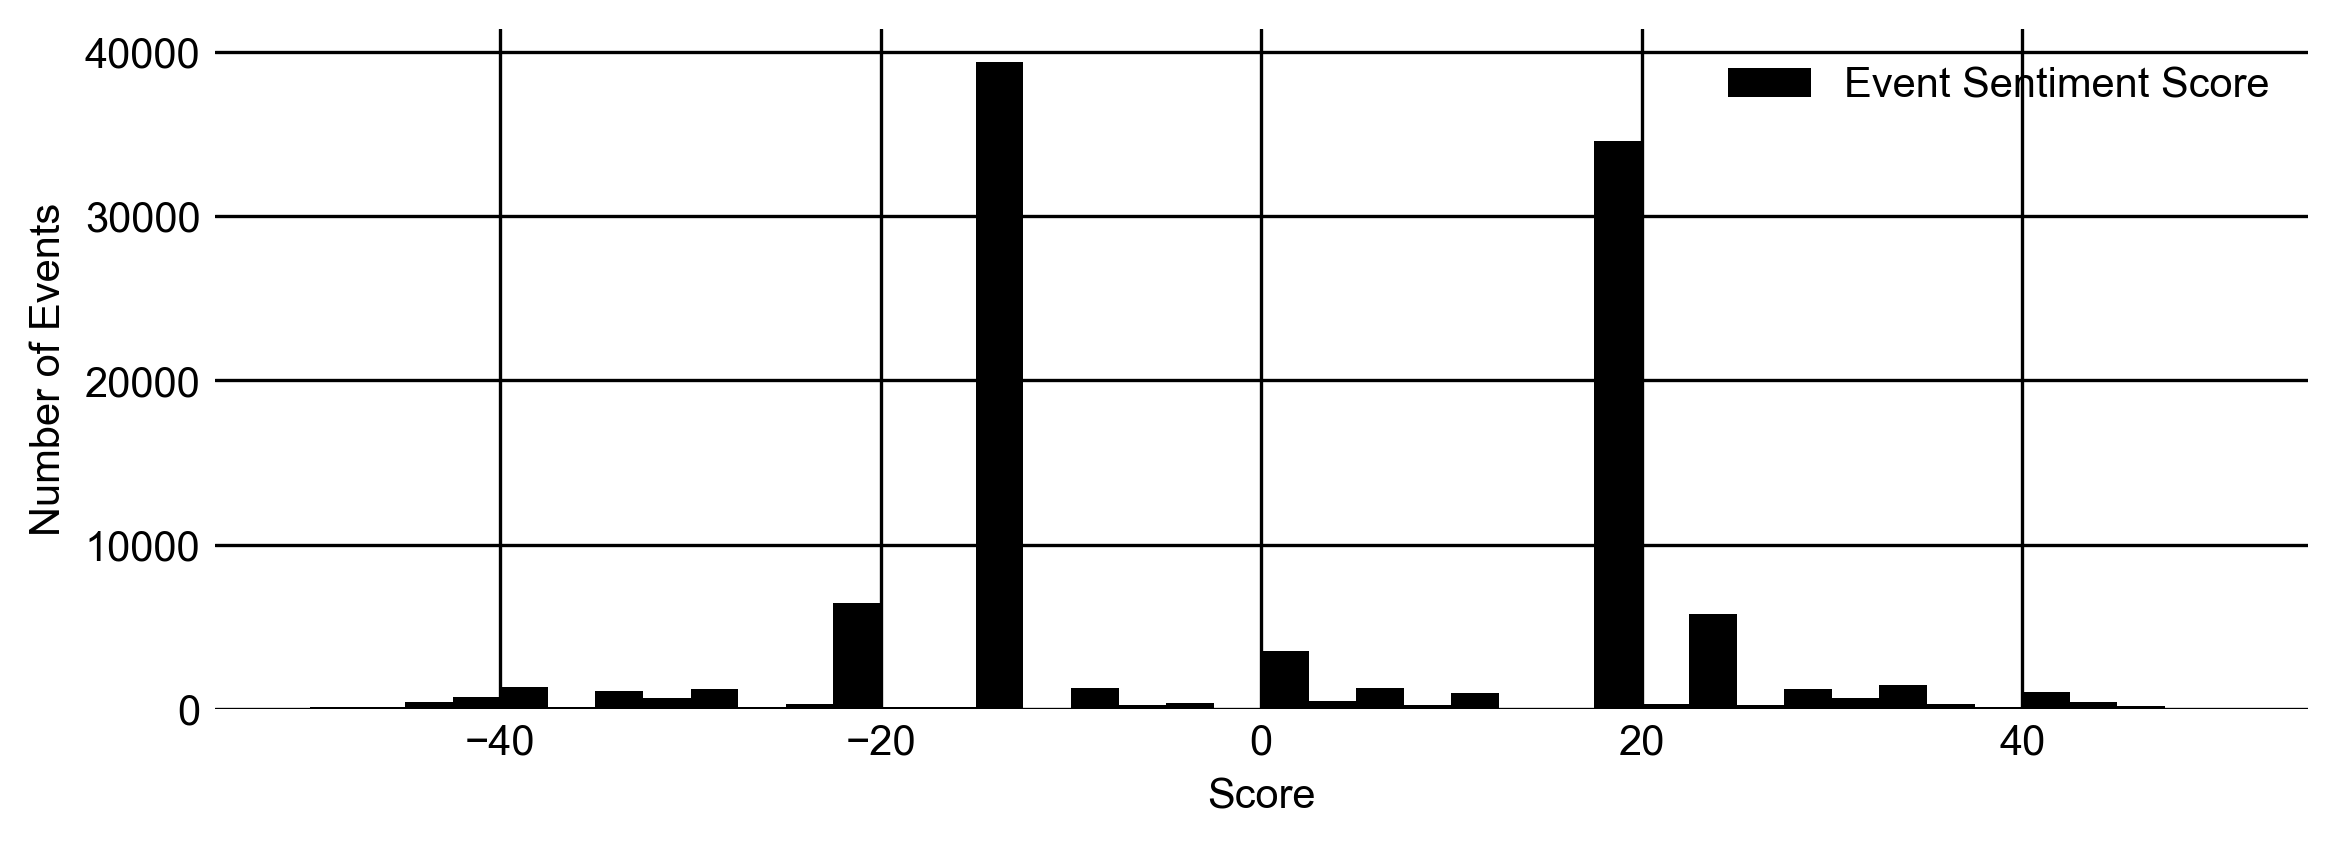
\includegraphics[width=\linewidth]{figures/event_classification/hist_ess_all.png}
		\caption{Distribution of Event Sentiment Scores of all 106,960 news items.}
	\end{figure}

	\par It is worth mentioning that ESS measures the potential impact on the topic of this news. For example, a civil unrest in a middle east country is often considered as news forerun negative economic impact, especially for the country itself.
	However, such news is in general associated with positive ESS scores because the expected negative supply shocks carried by these news are typically positively correlated crude oil prices and returns. \textbf{Tables below} present a list of categories frequently associated with positive and negatives news. From these two table we can see that the majority of themes of positive news would impact crude oil prices and returns positively.
	\begin{table}[H]
		\centering
		\small
		\begin{tabular}{l|c}
			\toprule
			Category & Number of positive news \\
			\midrule
			commodity-price-gain & 22,893 \\
			commodity-futures-gain & 11,648 \\
			supply-decrease-commodity & 5,845 \\
			imports-up & 2,705 \\
			commodity-buy-target & 1,171 \\
			demand-increase-commodity & 1,070 \\
			exports-down & 1,020 \\
			other 28 categories & 3,014 \\
			\midrule
			all positive news & 49,366 \\
			\bottomrule
		\end{tabular}
		\caption{Most frequent categories of positive news. Only categories with frequency greater than 1,000 are shown in this table.}
	\end{table}

	\begin{table}[H]
		\centering
		\small
		\begin{tabular}{l|c}
			\toprule
			Category & Number of negative news \\
			\midrule
			commodity-price-loss & 26,475 \\
			commodity-futures-loss & 12,818 \\
			supply-increase-commodity & 6,629 \\
			imports-down & 2,017 \\
			exports-up & 1308 \\
			resource-discovery-commodity & 1,179 \\
			technical-view-bearish & 1,172 \\
			other 24 categories & 2,517 \\
			\midrule
			all negative news & 54,115 \\
			\bottomrule
		\end{tabular}
		\caption{Most frequent categories of positive news. Only categories with frequency greater than 1,000 are shown in this table.}
	\end{table}
	
	\begin{table}[H]
		\centering
		\small
		\caption{Summary Statistics for Daily News Arrival by Years}
		\begin{tabular}{l | c c c c c c c}
		\toprule
		Year & Mean & Median & Std. & Min & Max & $3^{rd}$ Moment & $4^{th}$ Moment \\
		\midrule
2000 & 10.990 & 10.000 & 7.883 & 1.000 & 48.000 & 624.140 & 20580.847\\
2001 & 14.929 & 14.000 & 9.225 & 1.000 & 51.000 & 489.795 & 25704.202\\
2002 & 4.807 & 4.000 & 3.452 & 1.000 & 19.000 & 60.569 & 801.811\\
2003 & 6.519 & 4.000 & 6.241 & 1.000 & 39.000 & 478.654 & 12369.937\\
2004 & 24.608 & 23.000 & 16.612 & 1.000 & 84.000 & 3190.837 & 261755.365\\
2005 & 20.921 & 21.000 & 12.480 & 1.000 & 57.000 & 668.782 & 71292.410\\
2006 & 21.375 & 21.000 & 13.224 & 1.000 & 58.000 & 311.175 & 72550.280\\
2007 & 19.695 & 18.000 & 12.724 & 1.000 & 66.000 & 1080.233 & 80582.446\\
2008 & 22.264 & 23.000 & 14.481 & 1.000 & 66.000 & 773.619 & 114575.879\\
2009 & 16.642 & 16.000 & 10.145 & 1.000 & 48.000 & 229.465 & 26102.072\\
2010 & 17.373 & 18.000 & 10.704 & 1.000 & 52.000 & 223.408 & 32208.647\\
2011 & 22.252 & 23.000 & 12.838 & 1.000 & 65.000 & 346.488 & 76634.229\\
2012 & 22.679 & 23.000 & 13.582 & 1.000 & 65.000 & 327.492 & 89356.087\\
2013 & 17.048 & 17.000 & 10.419 & 1.000 & 57.000 & 405.999 & 35381.337\\
2014 & 16.193 & 13.000 & 13.162 & 1.000 & 69.000 & 3434.647 & 167509.547\\
2015 & 22.334 & 20.000 & 14.945 & 1.000 & 80.000 & 2368.778 & 171467.903\\
2016 & 24.361 & 22.000 & 16.265 & 1.000 & 101.000 & 3602.310 & 285093.246\\
2017 & 15.428 & 14.000 & 10.105 & 1.000 & 58.000 & 815.307 & 43032.009\\
2018 & 15.692 & 15.000 & 10.870 & 1.000 & 93.000 & 1976.611 & 145822.537\\
2019 & 15.157 & 14.000 & 9.584 & 1.000 & 65.000 & 968.021 & 47684.600\\
		\bottomrule
		\end{tabular}
	\end{table}
	
	\begin{table}[H]
		\centering
		\small
		\caption{Average Numbers of News on Each Day}
		\begin{tabular}{l|c c c c c c c}
			\toprule
			Year & Monday &Tuesday &Wednesday &Thursday &Friday &Saturday &Sunday \\ 
			\midrule
2000 & 11.157 & 14.135 & 13.077 & 11.885 & 9.769 & 1.643 & 1.500 \\
2001 & 12.547 & 17.569 & 21.327 & 15.058 & 14.078 & 1.000 & 1.200 \\
2002 & 5.771 & 5.019 & 5.224 & 3.980 & 5.469 & 1.200 & 1.600 \\
2003 & 7.080 & 6.529 & 9.942 & 6.863 & 5.490 & 1.200 & 1.136 \\
2004 & 24.058 & 28.981 & 39.250 & 28.660 & 22.302 & 2.182 & 2.240 \\
2005 & 21.462 & 21.846 & 33.596 & 24.654 & 19.000 & 1.765 & 2.259 \\
2006 & 22.981 & 24.885 & 35.904 & 24.846 & 19.731 & 1.346 & 2.161 \\
2007 & 19.792 & 21.385 & 33.577 & 23.846 & 16.769 & 1.941 & 2.212 \\
2008 & 24.788 & 26.415 & 36.415 & 26.269 & 25.250 & 2.207 & 3.065 \\
2009 & 16.058 & 21.346 & 29.192 & 16.925 & 15.538 & 1.688 & 2.366 \\
2010 & 16.327 & 23.058 & 28.654 & 20.596 & 17.135 & 2.261 & 2.932 \\
2011 & 23.769 & 28.577 & 32.904 & 25.750 & 19.942 & 2.053 & 3.441 \\
2012 & 22.340 & 26.654 & 36.423 & 26.981 & 25.118 & 3.783 & 2.756 \\
2013 & 16.673 & 19.642 & 28.588 & 19.038 & 15.846 & 2.500 & 2.366 \\
2014 & 15.510 & 18.846 & 25.113 & 16.923 & 15.529 & 2.167 & 2.467 \\
2015 & 23.019 & 27.135 & 35.558 & 23.189 & 19.843 & 2.091 & 2.957 \\
2016 & 23.333 & 29.192 & 38.462 & 24.808 & 23.077 & 2.190 & 2.105 \\
2017 & 14.220 & 16.788 & 25.192 & 16.077 & 14.039 & 1.696 & 1.667 \\
2018 & 13.654 & 19.059 & 24.712 & 18.635 & 15.235 & 2.586 & 2.143 \\
2019 & 11.263 & 15.872 & 24.600 & 15.026 & 13.795 & 1.923 & 1.500 \\
		\bottomrule
		\end{tabular}
	\end{table}

	\subsection{Classifying News Type}
	
	\subsection{Case Studies of Events}
	\subsubsection{Positive Spike on November 30, 2016}
	\begin{figure}[H]
		\centering
		\small
		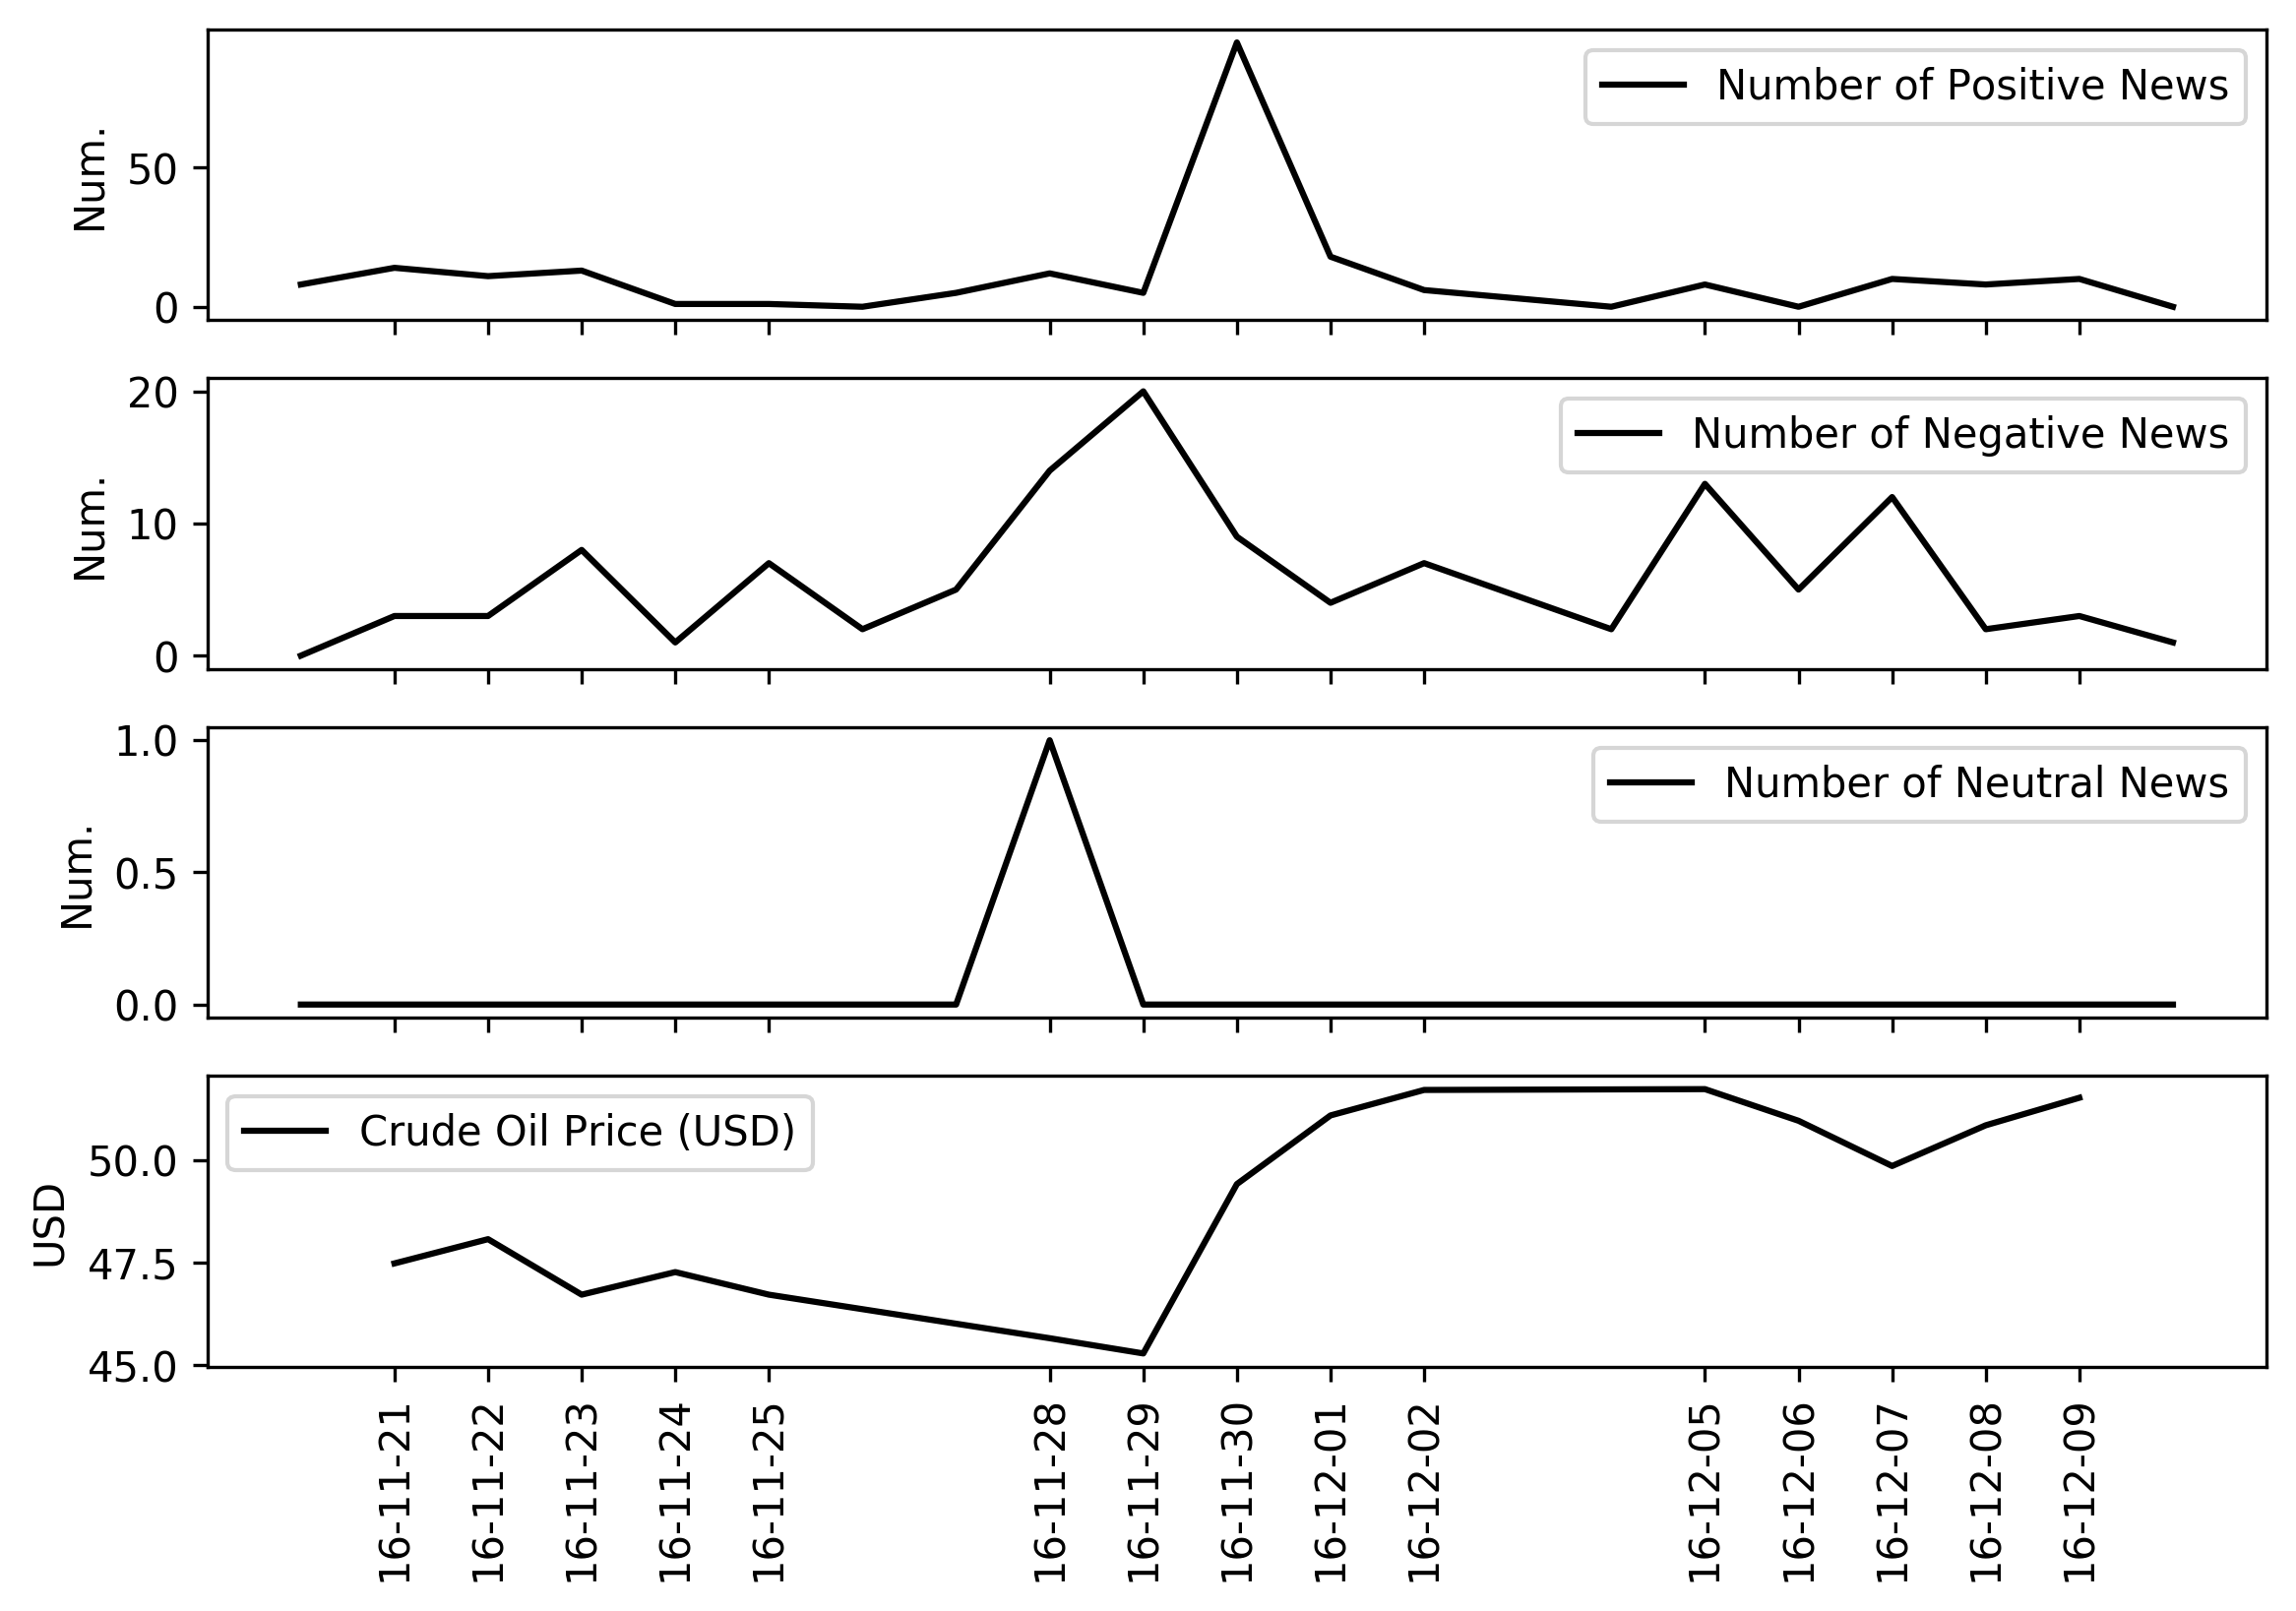
\includegraphics[width=\linewidth]{figures/case_studies/20161130_10d.png}
		\caption{}
	\end{figure}
	
	\subsubsection{Negative Spike on December 6, 2018}
	\begin{figure}[H]
		\centering
		\small
		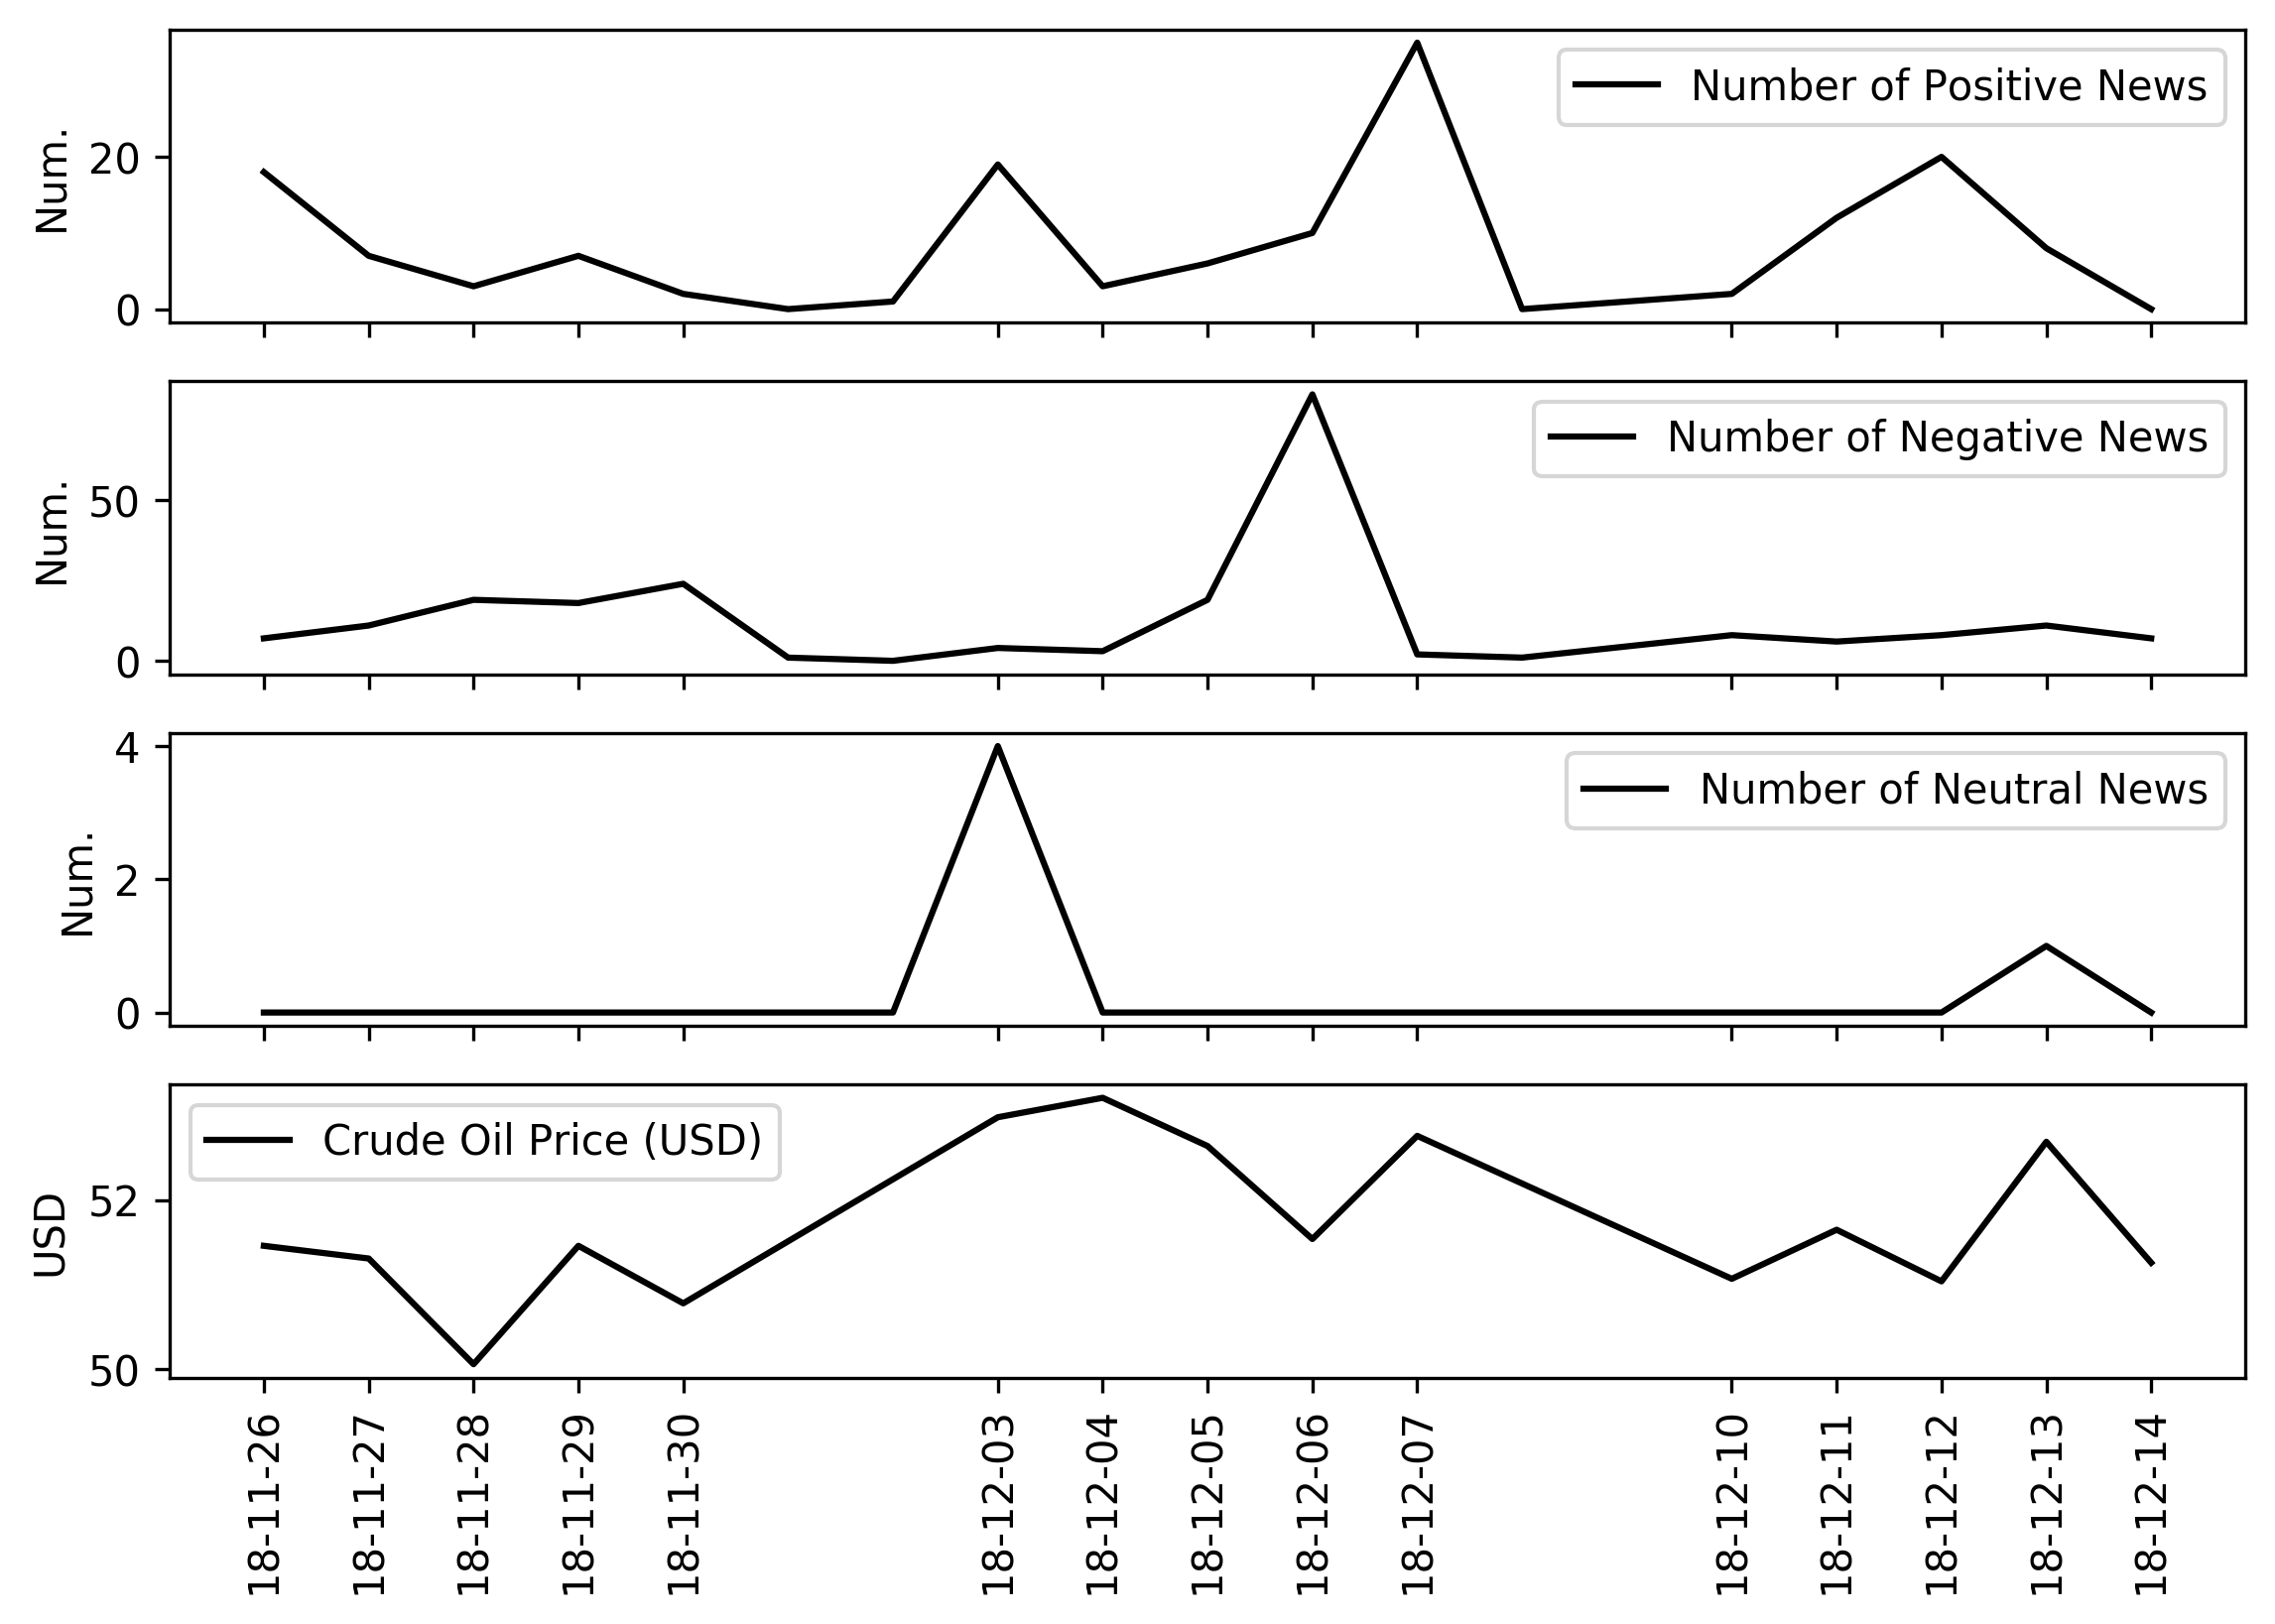
\includegraphics[width=\linewidth]{figures/case_studies/20181206_10d.png}
		\caption{}
	\end{figure}
	
	\subsubsection{Positive Spike on June. 12 - 13, 2019}
	\begin{figure}[H]
		\centering
		\small
		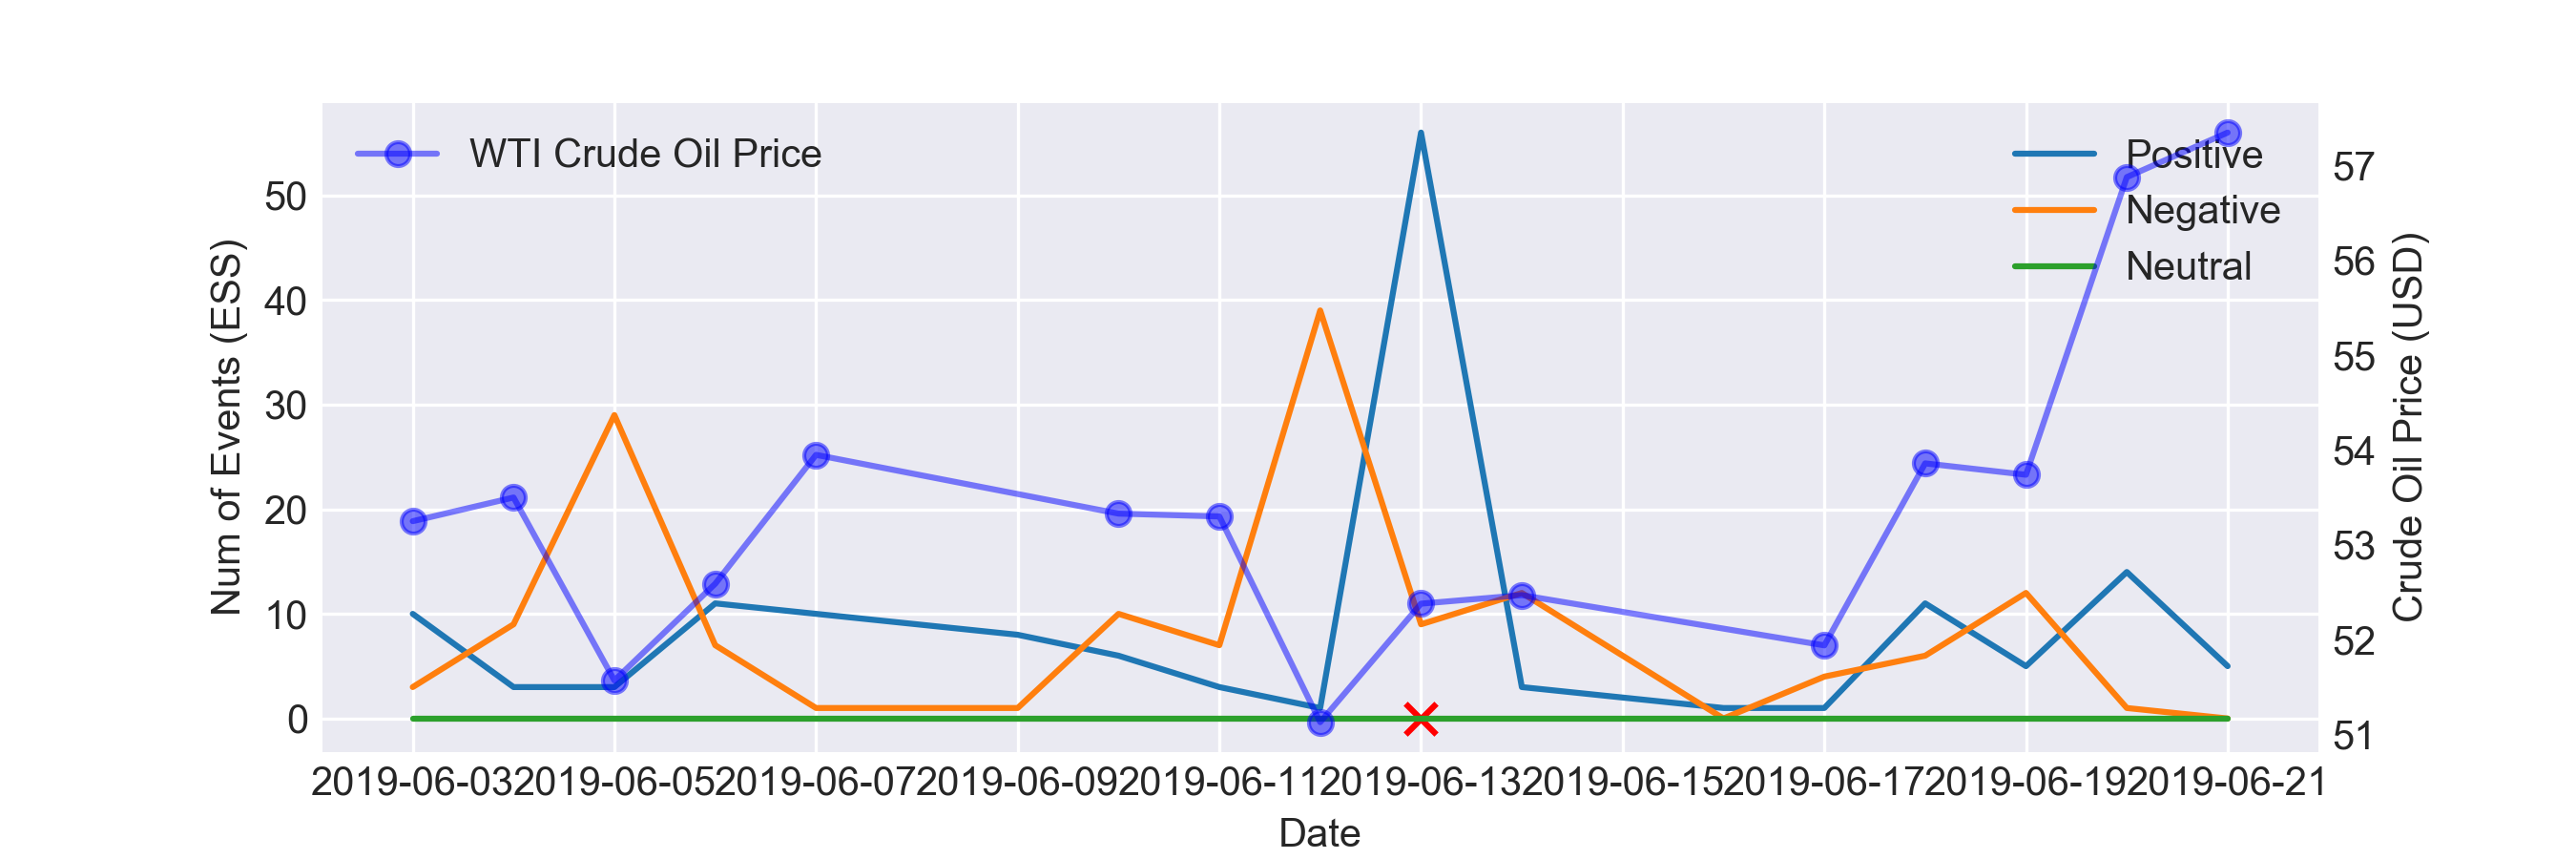
\includegraphics[width=\linewidth]{figures/case_studies/20190612_10d.png}
		\caption{}
	\end{figure}
	\section{Models}
	
	\section{Experiments}

	% Bib
	\bibliographystyle{apacite}
	
	\bibliography{thesis.bib}

%	\section{Appendix: Supplementary Summary Statistics for Datasets}
%	
%	\begin{figure}[H]
%		\centering
%		\small
%		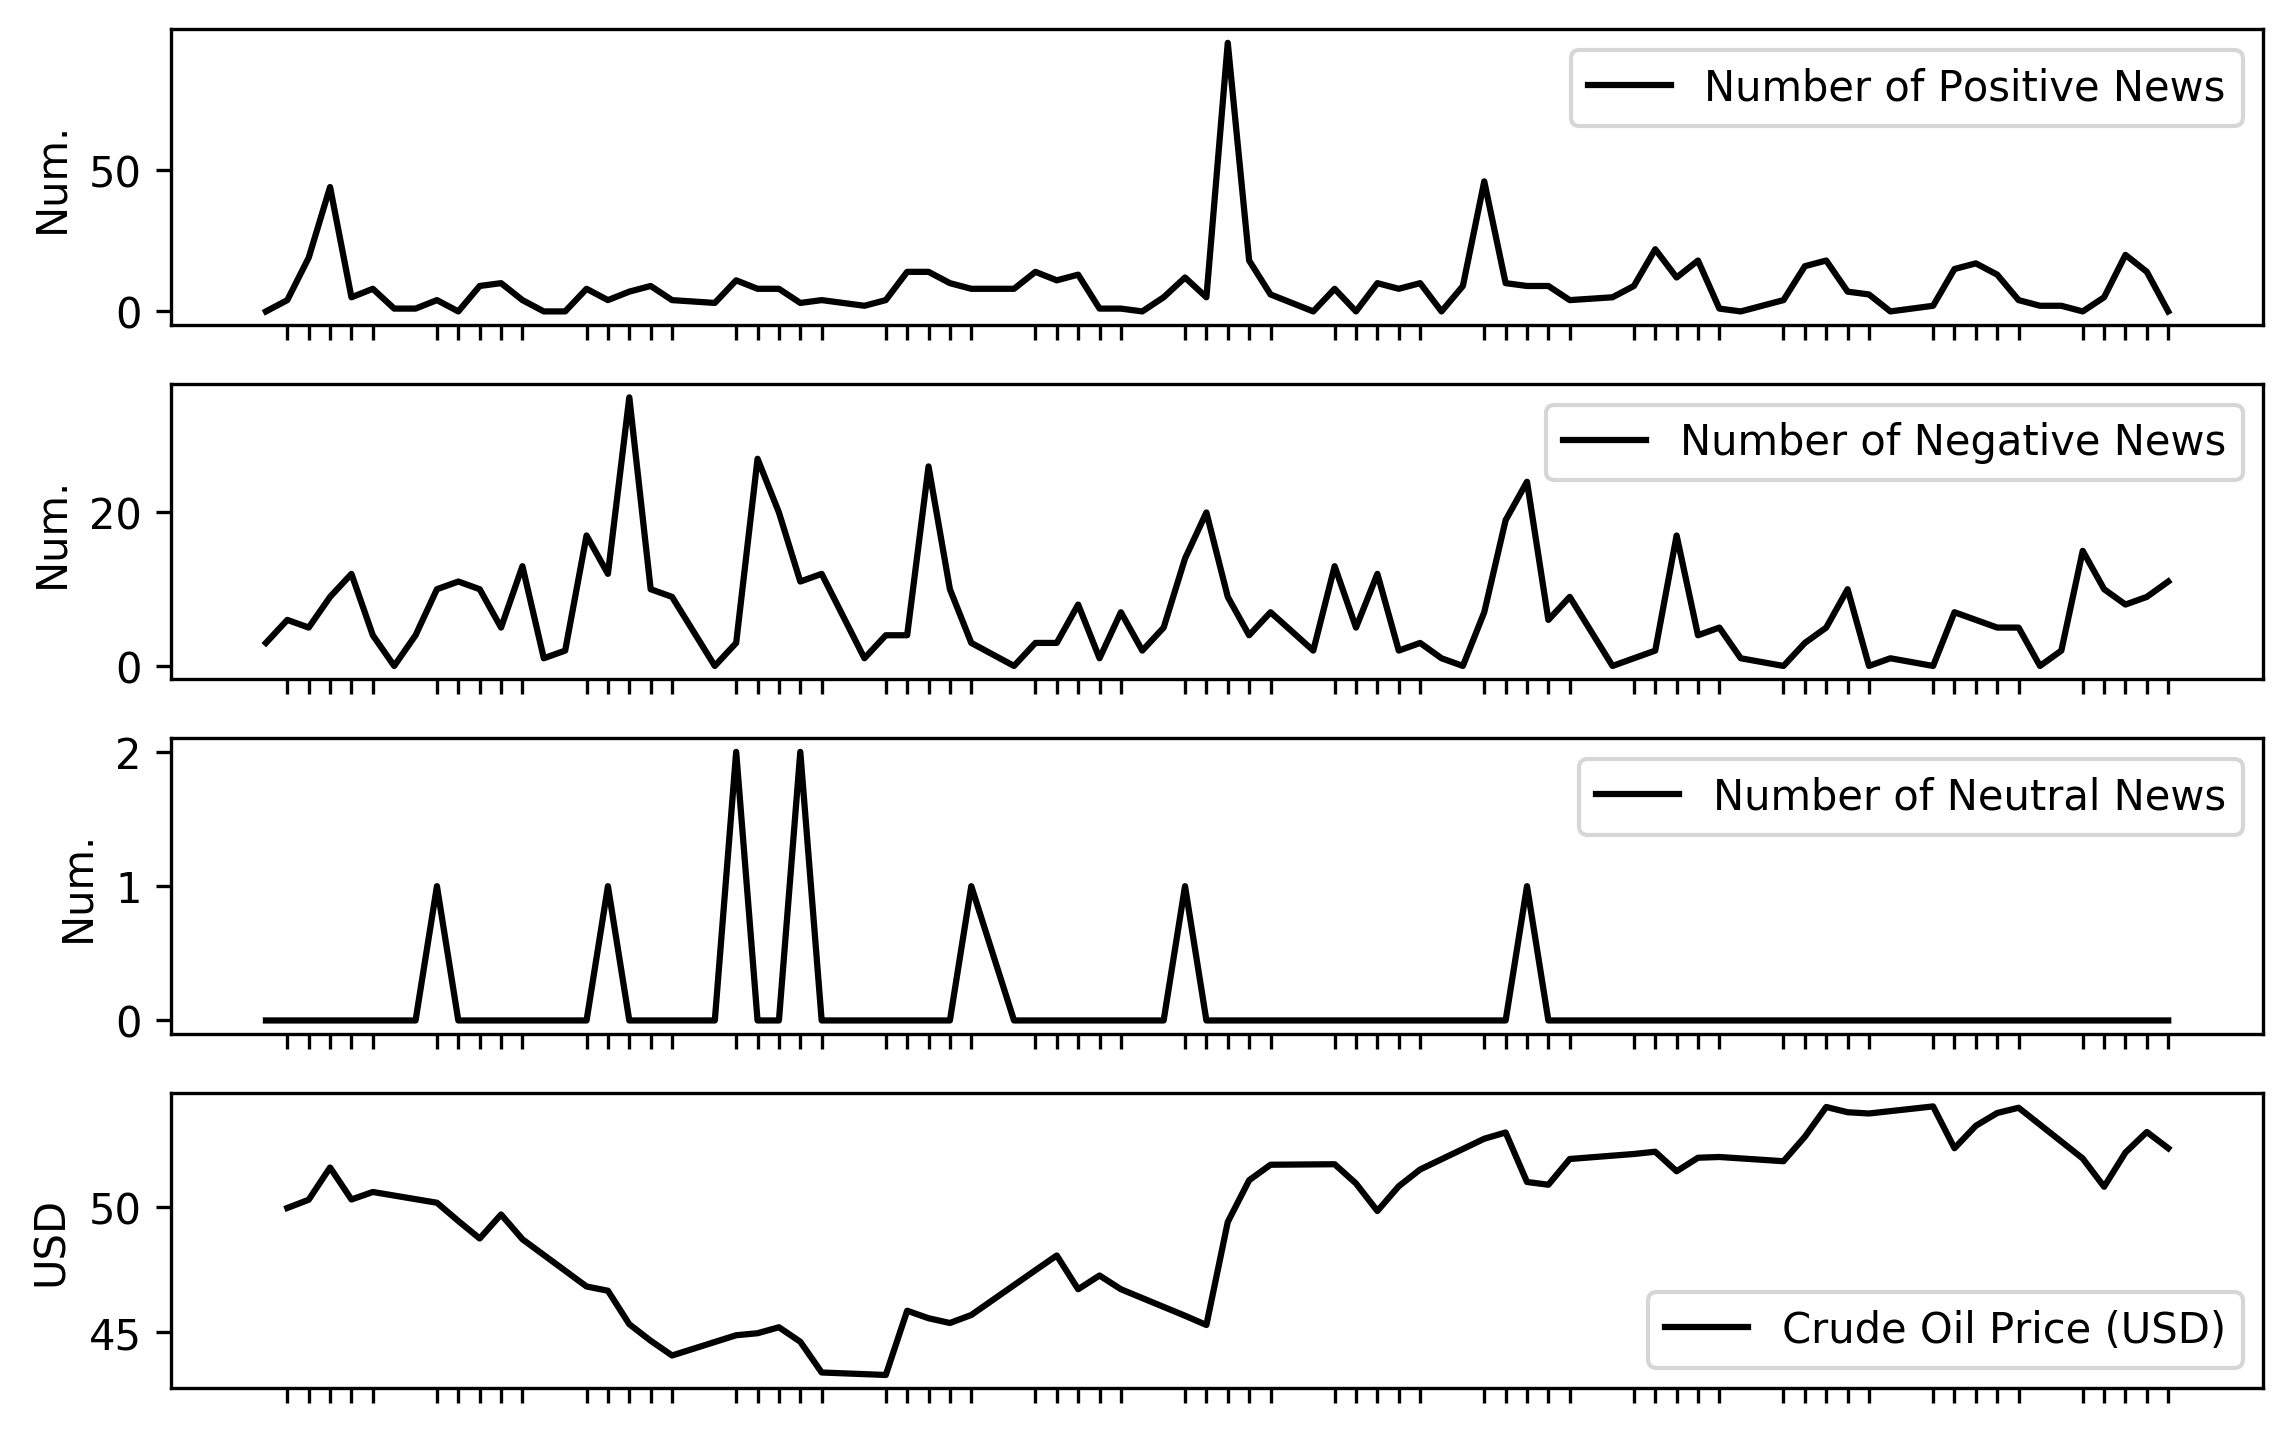
\includegraphics[width=\linewidth]{figures/case_studies/20161130_45d.png}
%		\caption{}
%	\end{figure}
%	\begin{figure}[H]
%		\centering
%		\small
%		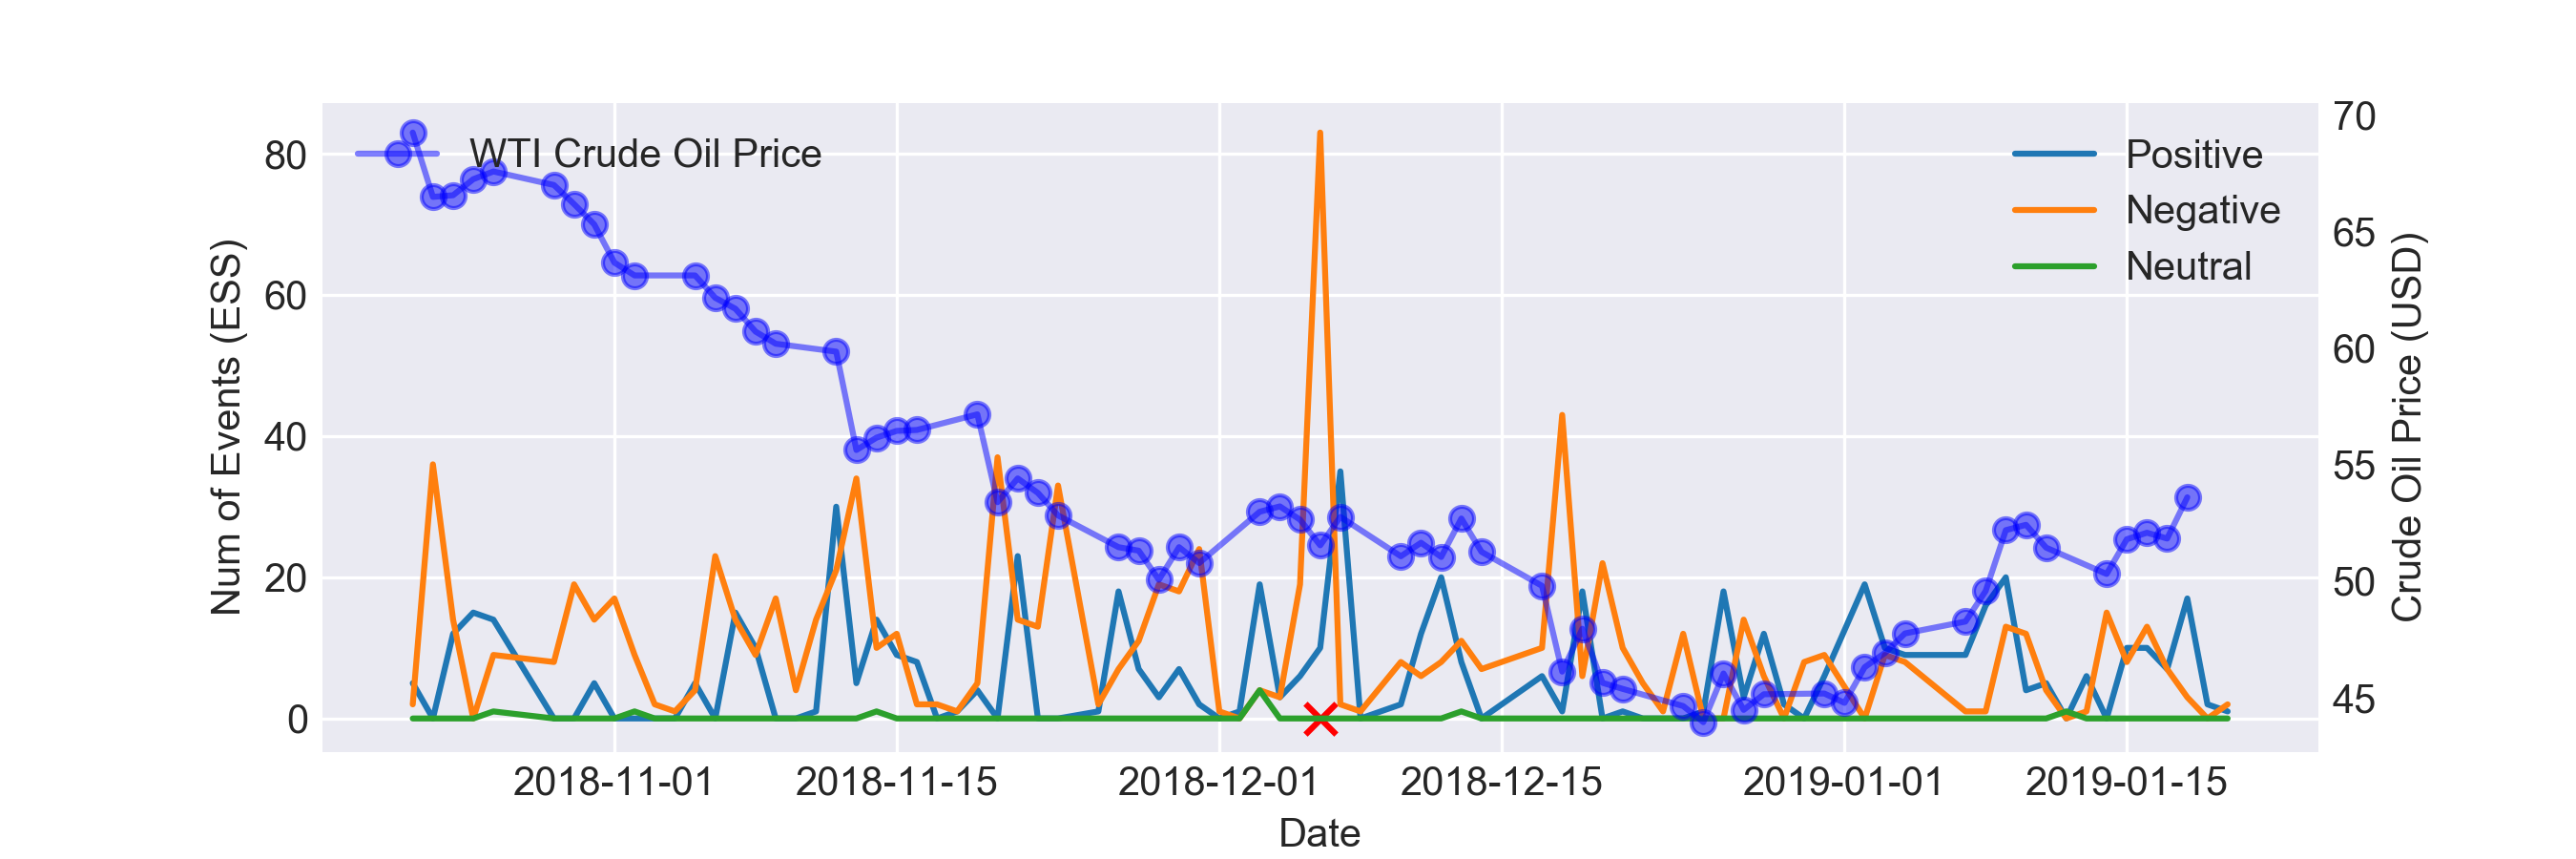
\includegraphics[width=\linewidth]{figures/case_studies/20181206_45d.png}
%		\caption{}
%	\end{figure}
%	\begin{figure}[H]
%		\centering
%		\small
%		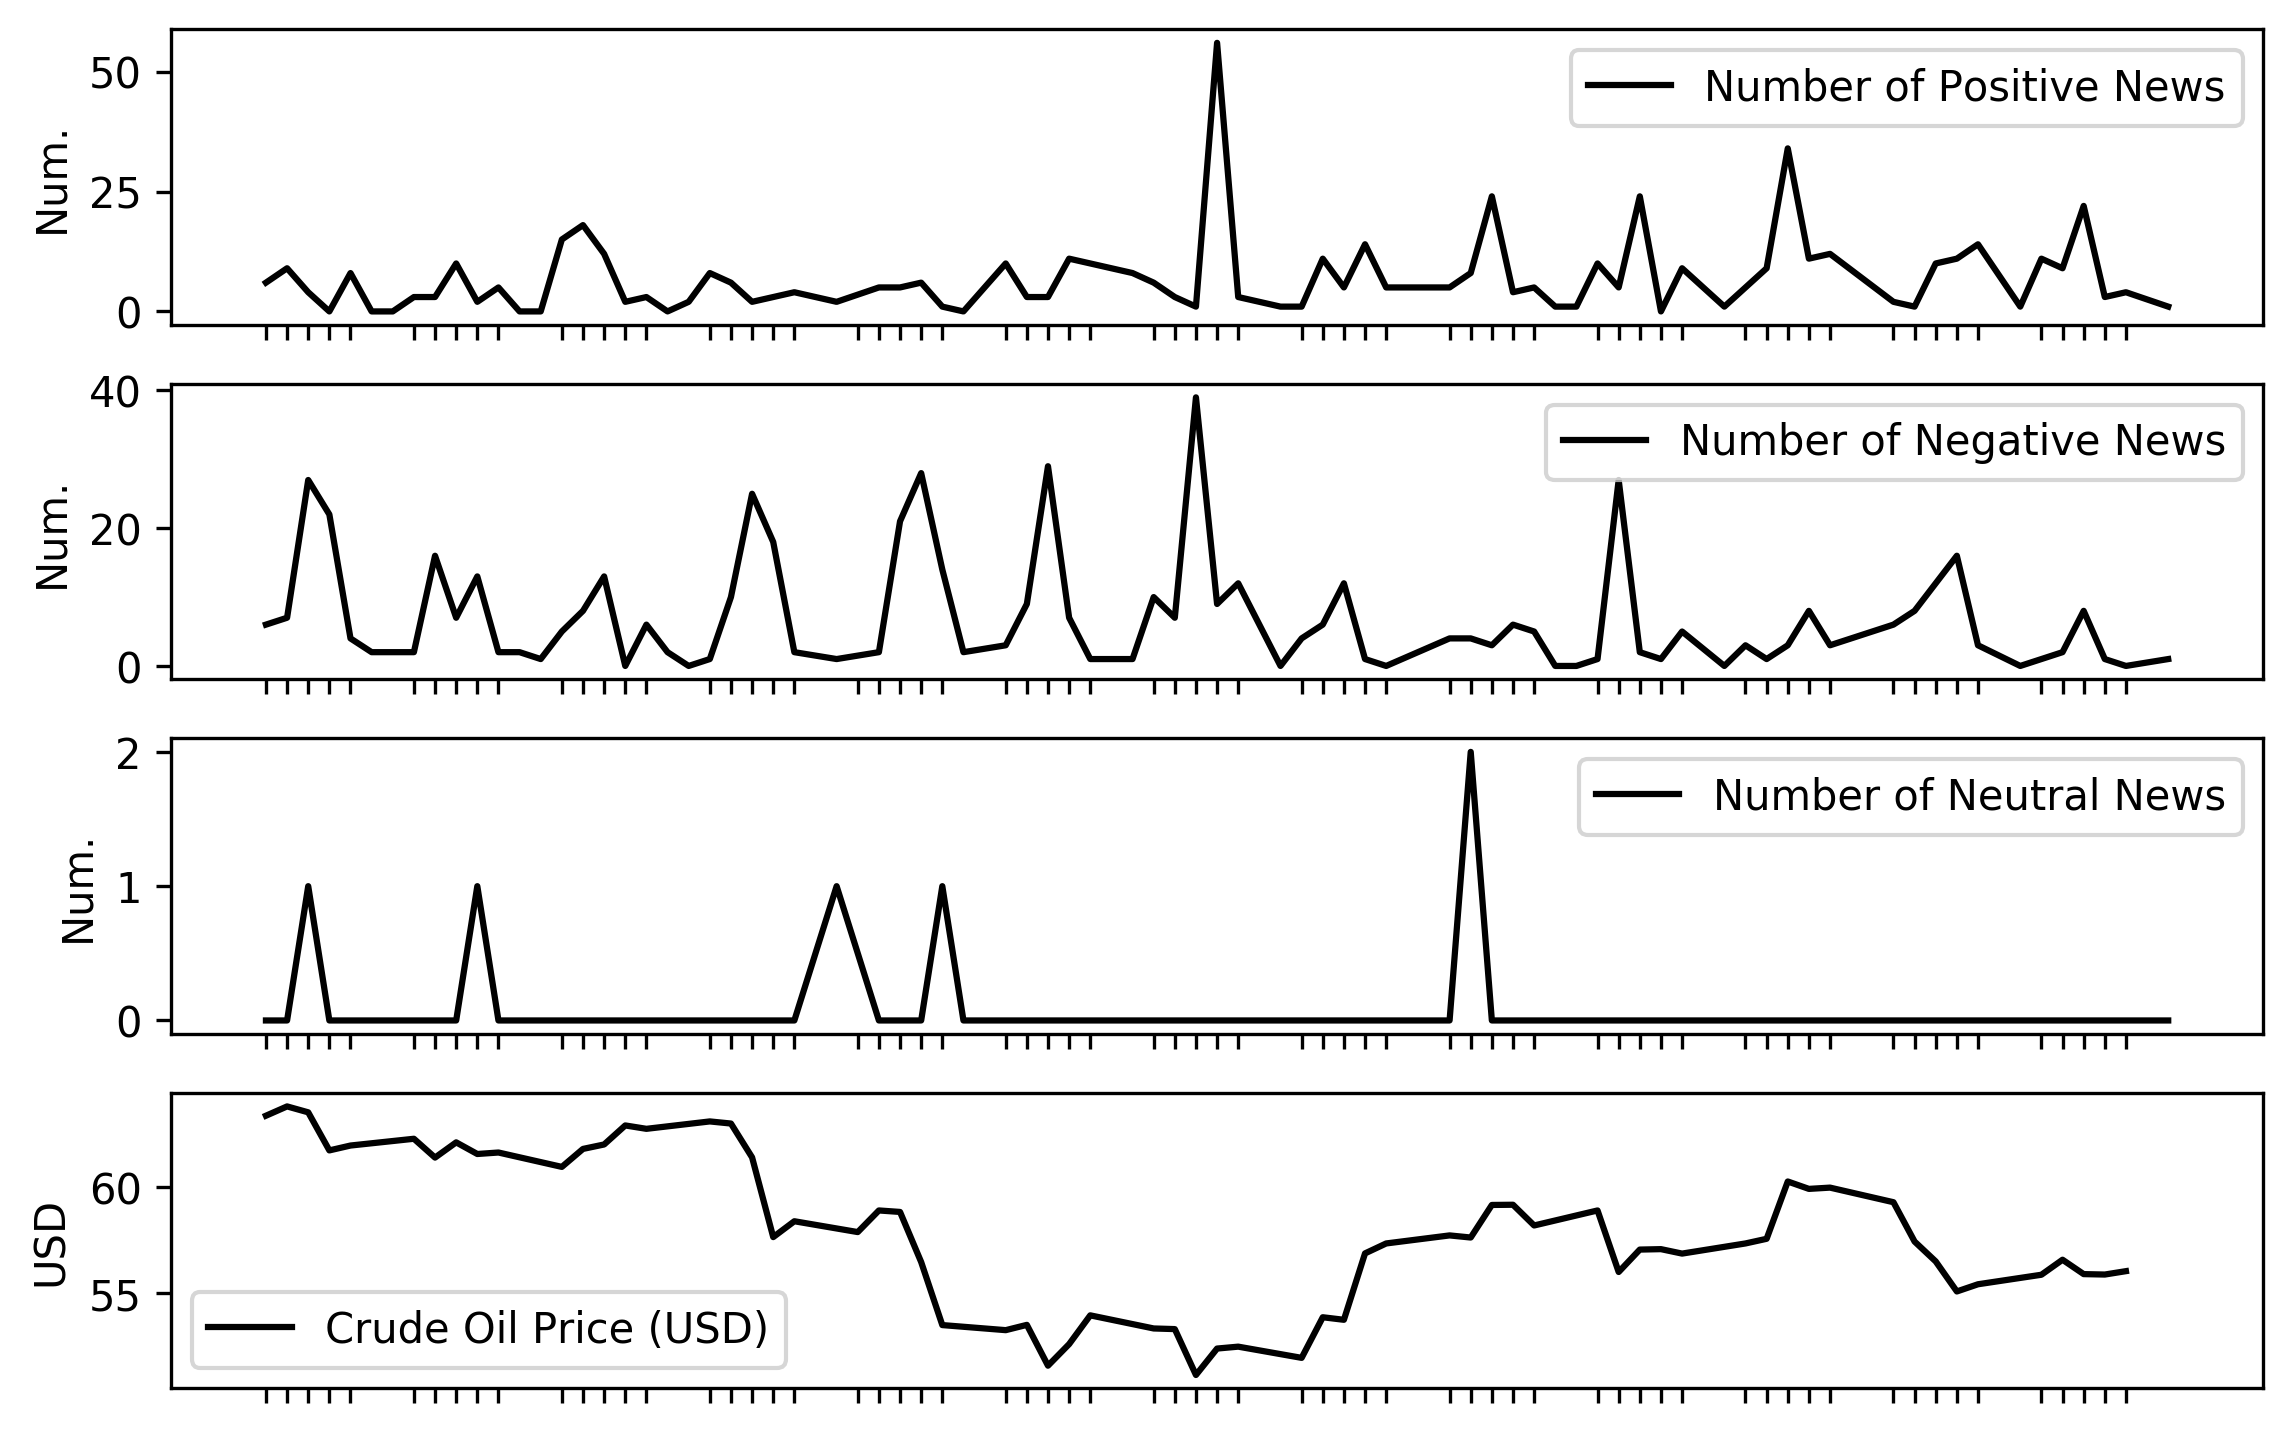
\includegraphics[width=\linewidth]{figures/case_studies/20190612_45d.png}
%		\caption{}
%	\end{figure}


\end{document}
























